\documentclass[11pt,a4paper]{article}

\usepackage[margin=1in]{geometry}
\usepackage{titlesec}
\usepackage{enumitem}
\usepackage{hyperref}
\usepackage{xcolor}
\usepackage{fancyhdr}
\usepackage{booktabs}
\usepackage{array}
\usepackage{graphicx}
\usepackage{float}
\usepackage{multirow}
\usepackage{parskip}

\definecolor{darkblue}{RGB}{20, 60, 140}
\definecolor{darkgreen}{RGB}{0, 100, 70}
\definecolor{lightgray}{RGB}{245, 245, 245}
\definecolor{borderblue}{RGB}{180, 200, 235}

\hypersetup{
    colorlinks=true,
    linkcolor=darkblue,
    urlcolor=darkblue,
    citecolor=darkblue
}

\pagestyle{fancy}
\fancyhf{}
\setlength{\headheight}{14pt}
\addtolength{\topmargin}{-2pt}
\rhead{\textcolor{darkblue}{\small MLOps Group Assignment --- Group 13}}
\lhead{\textcolor{gray}{\small IIT Jodhpur | PGD AI Program}}
\rfoot{\textcolor{gray}{\small \thepage}}
\renewcommand{\headrulewidth}{0.4pt}

\titleformat{\section}{\large\bfseries\color{darkblue}}{}{0em}{\arabic{section}.\ }[\titlerule]
\titleformat{\subsection}{\normalsize\bfseries\color{darkgreen}}{}{0em}{\thesubsection\ }

\setlength{\parskip}{5pt}
\setlength{\parindent}{0pt}

\newcommand{\screenshotbox}[1]{%
  \begin{center}
  \fbox{\parbox{0.85\textwidth}{\centering\vspace{0.5cm}
  \textbf{[SCREENSHOT: #1]}\vspace{0.5cm}}}
  \end{center}
}

% -----------------------------------------------------------
\begin{document}

% ======================== TITLE PAGE ========================
\begin{titlepage}
\centering
\vspace*{2cm}

{\color{darkblue}\rule{\linewidth}{2pt}}\\[0.4cm]
{\LARGE\bfseries\color{darkblue} MLOps Group Assignment}\\[0.3cm]
{\large AG News Text Classification Pipeline}\\[0.2cm]
{\normalsize Fine-tuning DistilBERT with Docker, CI/CD, and W\&B Tracking}\\[0.4cm]
{\color{darkblue}\rule{\linewidth}{2pt}}

\vspace{1.5cm}

\renewcommand{\arraystretch}{1.5}
\begin{tabular}{ll}
\textbf{Course:}         & MLOps | PGD AI Program \\
\textbf{Institute:}      & IIT Jodhpur \\
\textbf{Group Number:}   & Group 13 \\
\textbf{Submission Date:} & June 2026 \\
\end{tabular}

\vspace{1.2cm}

\renewcommand{\arraystretch}{1.4}
\begin{tabular}{lll}
\hline
\textbf{Name} & \textbf{Roll Number} & \textbf{Contribution} \\
\hline
Ritesh Maury               & G25AIT2087 & GitHub Setup, Project Lead, Merges \\
Kosuru Yuvaraj             & G25AIT2054 & Training, Docker, CI/CD, HF Hub, Report \\
Laishram Khumanleima Chanu & G25AIT2056 & Data Preparation, Inference Script \\
Guntakal Sandeep Kumar     & G25AIT2036 & W\&B Tracking, Evaluation, Testing \\
\hline
\end{tabular}

\vspace{1.5cm}

\textbf{\large All Submission Links}\\[0.4cm]
\renewcommand{\arraystretch}{1.5}
\begin{tabular}{ll}
\textbf{GitHub Repository:} & \href{https://github.com/riteshmaury-iitj/group13-assignment-mlops}{\texttt{riteshmaury-iitj/group13-assignment-mlops}} \\
\textbf{Kaggle Notebook V1:} & \href{https://www.kaggle.com/code/kyuvarajg25ait2054/group13-ag-news-k}{\texttt{kyuvarajg25ait2054/group13-ag-news-k}} \\
\textbf{Kaggle Notebook V2:} & \href{https://www.kaggle.com/code/kyuvarajg25ait2054/group13-ag-news-k}{\texttt{kyuvarajg25ait2054/group13-ag-news-k}} \\
\textbf{HuggingFace Model:} & \href{https://huggingface.co/YuvarajK-g25ait2054/ag-news-distilbert}{\texttt{YuvarajK-g25ait2054/ag-news-distilbert}} \\
\textbf{Docker Image:}      & \href{https://hub.docker.com/r/yuvarajkg25ait2054/ag-news-classifier}{\texttt{yuvarajkg25ait2054/ag-news-classifier}} \\
\textbf{W\&B Dashboard:}    & \href{https://wandb.ai/g25ait2054-iit-jodhpur/mlops-assignment3}{\texttt{g25ait2054-iit-jodhpur/mlops-assignment3}} \\
\end{tabular}

\end{titlepage}

% ======================== MEMBER PROFILES & PROJECT LINKS ========================
\thispagestyle{fancy}

\begin{center}
{\large\bfseries\color{darkblue} Member Profiles \& Project Links}\\[0.2cm]
{\small All links are public and live at submission time.}
\end{center}

\vspace{0.4cm}

{\bfseries\color{darkgreen} Member Profiles}

\vspace{0.2cm}
\renewcommand{\arraystretch}{1.4}
\begin{tabular}{p{3.2cm}p{2.8cm}p{3cm}p{3.5cm}p{2.5cm}}
\toprule
\textbf{Member} & \textbf{GitHub} & \textbf{Kaggle} & \textbf{HuggingFace} & \textbf{W\&B} \\
\midrule
Ritesh Maury \newline G25AIT2087 &
  \href{https://github.com/riteshmaury-iitj}{\small riteshmaury-iitj} &
  {\small ---} & {\small ---} & {\small ---} \\
Kosuru Yuvaraj \newline G25AIT2054 &
  \href{https://github.com/yuvarajkosuru}{\small yuvarajkosuru} &
  \href{https://www.kaggle.com/kyuvarajg25ait2054}{\small kyuvarajg25ait2054} &
  \href{https://huggingface.co/YuvarajK-g25ait2054}{\small YuvarajK-g25ait2054} &
  \href{https://wandb.ai/g25ait2054-iit-jodhpur}{\small g25ait2054} \\
Laishram K. Chanu \newline G25AIT2056 &
  {\small ---} & {\small ---} & {\small ---} & {\small ---} \\
Guntakal Sandeep \newline G25AIT2036 &
  {\small ---} & {\small ---} & {\small ---} & {\small ---} \\
\bottomrule
\end{tabular}

\vspace{0.5cm}

{\bfseries\color{darkgreen} Project Links (all public)}

\vspace{0.2cm}
\renewcommand{\arraystretch}{1.4}
\begin{tabular}{p{5cm}p{9.5cm}}
\toprule
\textbf{Component} & \textbf{Link} \\
\midrule
GitHub Repository (public) & \href{https://github.com/riteshmaury-iitj/group13-assignment-mlops}{\small\texttt{github.com/riteshmaury-iitj/group13-assignment-mlops}} \\
Kaggle Notebook --- Version 1 (public) & \href{https://www.kaggle.com/code/kyuvarajg25ait2054/group13-ag-news-k}{\small\texttt{kaggle.com/code/kyuvarajg25ait2054/group13-ag-news-k}} \\
Kaggle Notebook --- Version 2 (public) & \href{https://www.kaggle.com/code/kyuvarajg25ait2054/group13-ag-news-k}{\small\texttt{kaggle.com/code/kyuvarajg25ait2054/group13-ag-news-k}} \\
HuggingFace Model (public) & \href{https://huggingface.co/YuvarajK-g25ait2054/ag-news-distilbert}{\small\texttt{huggingface.co/YuvarajK-g25ait2054/ag-news-distilbert}} \\
Docker Image (publicly pullable) & \href{https://hub.docker.com/r/yuvarajkg25ait2054/ag-news-classifier}{\small\texttt{hub.docker.com/r/yuvarajkg25ait2054/ag-news-classifier}} \\
W\&B Project Dashboard (public) & \href{https://wandb.ai/g25ait2054-iit-jodhpur/mlops-assignment3}{\small\texttt{wandb.ai/g25ait2054-iit-jodhpur/mlops-assignment3}} \\
\bottomrule
\end{tabular}

\newpage

% ======================== PAGE 2 ========================
\section{GitHub Repository, Data Preparation and Model Selection (Tasks 1--3)}

\subsection{Task 1 --- GitHub Repository Setup [10 marks]}

Repository \href{https://github.com/riteshmaury-iitj/group13-assignment-mlops}{\texttt{riteshmaury-iitj/group13-assignment-mlops}} is public with three branches: \textbf{main} (protected, PRs only), \textbf{develop} (integration), and \textbf{feature/*} (short-lived). Branch protection on \texttt{main} requires at least one approval before merging. All work was merged via Pull Request from \texttt{develop}.

\begin{figure}[H]
\centering
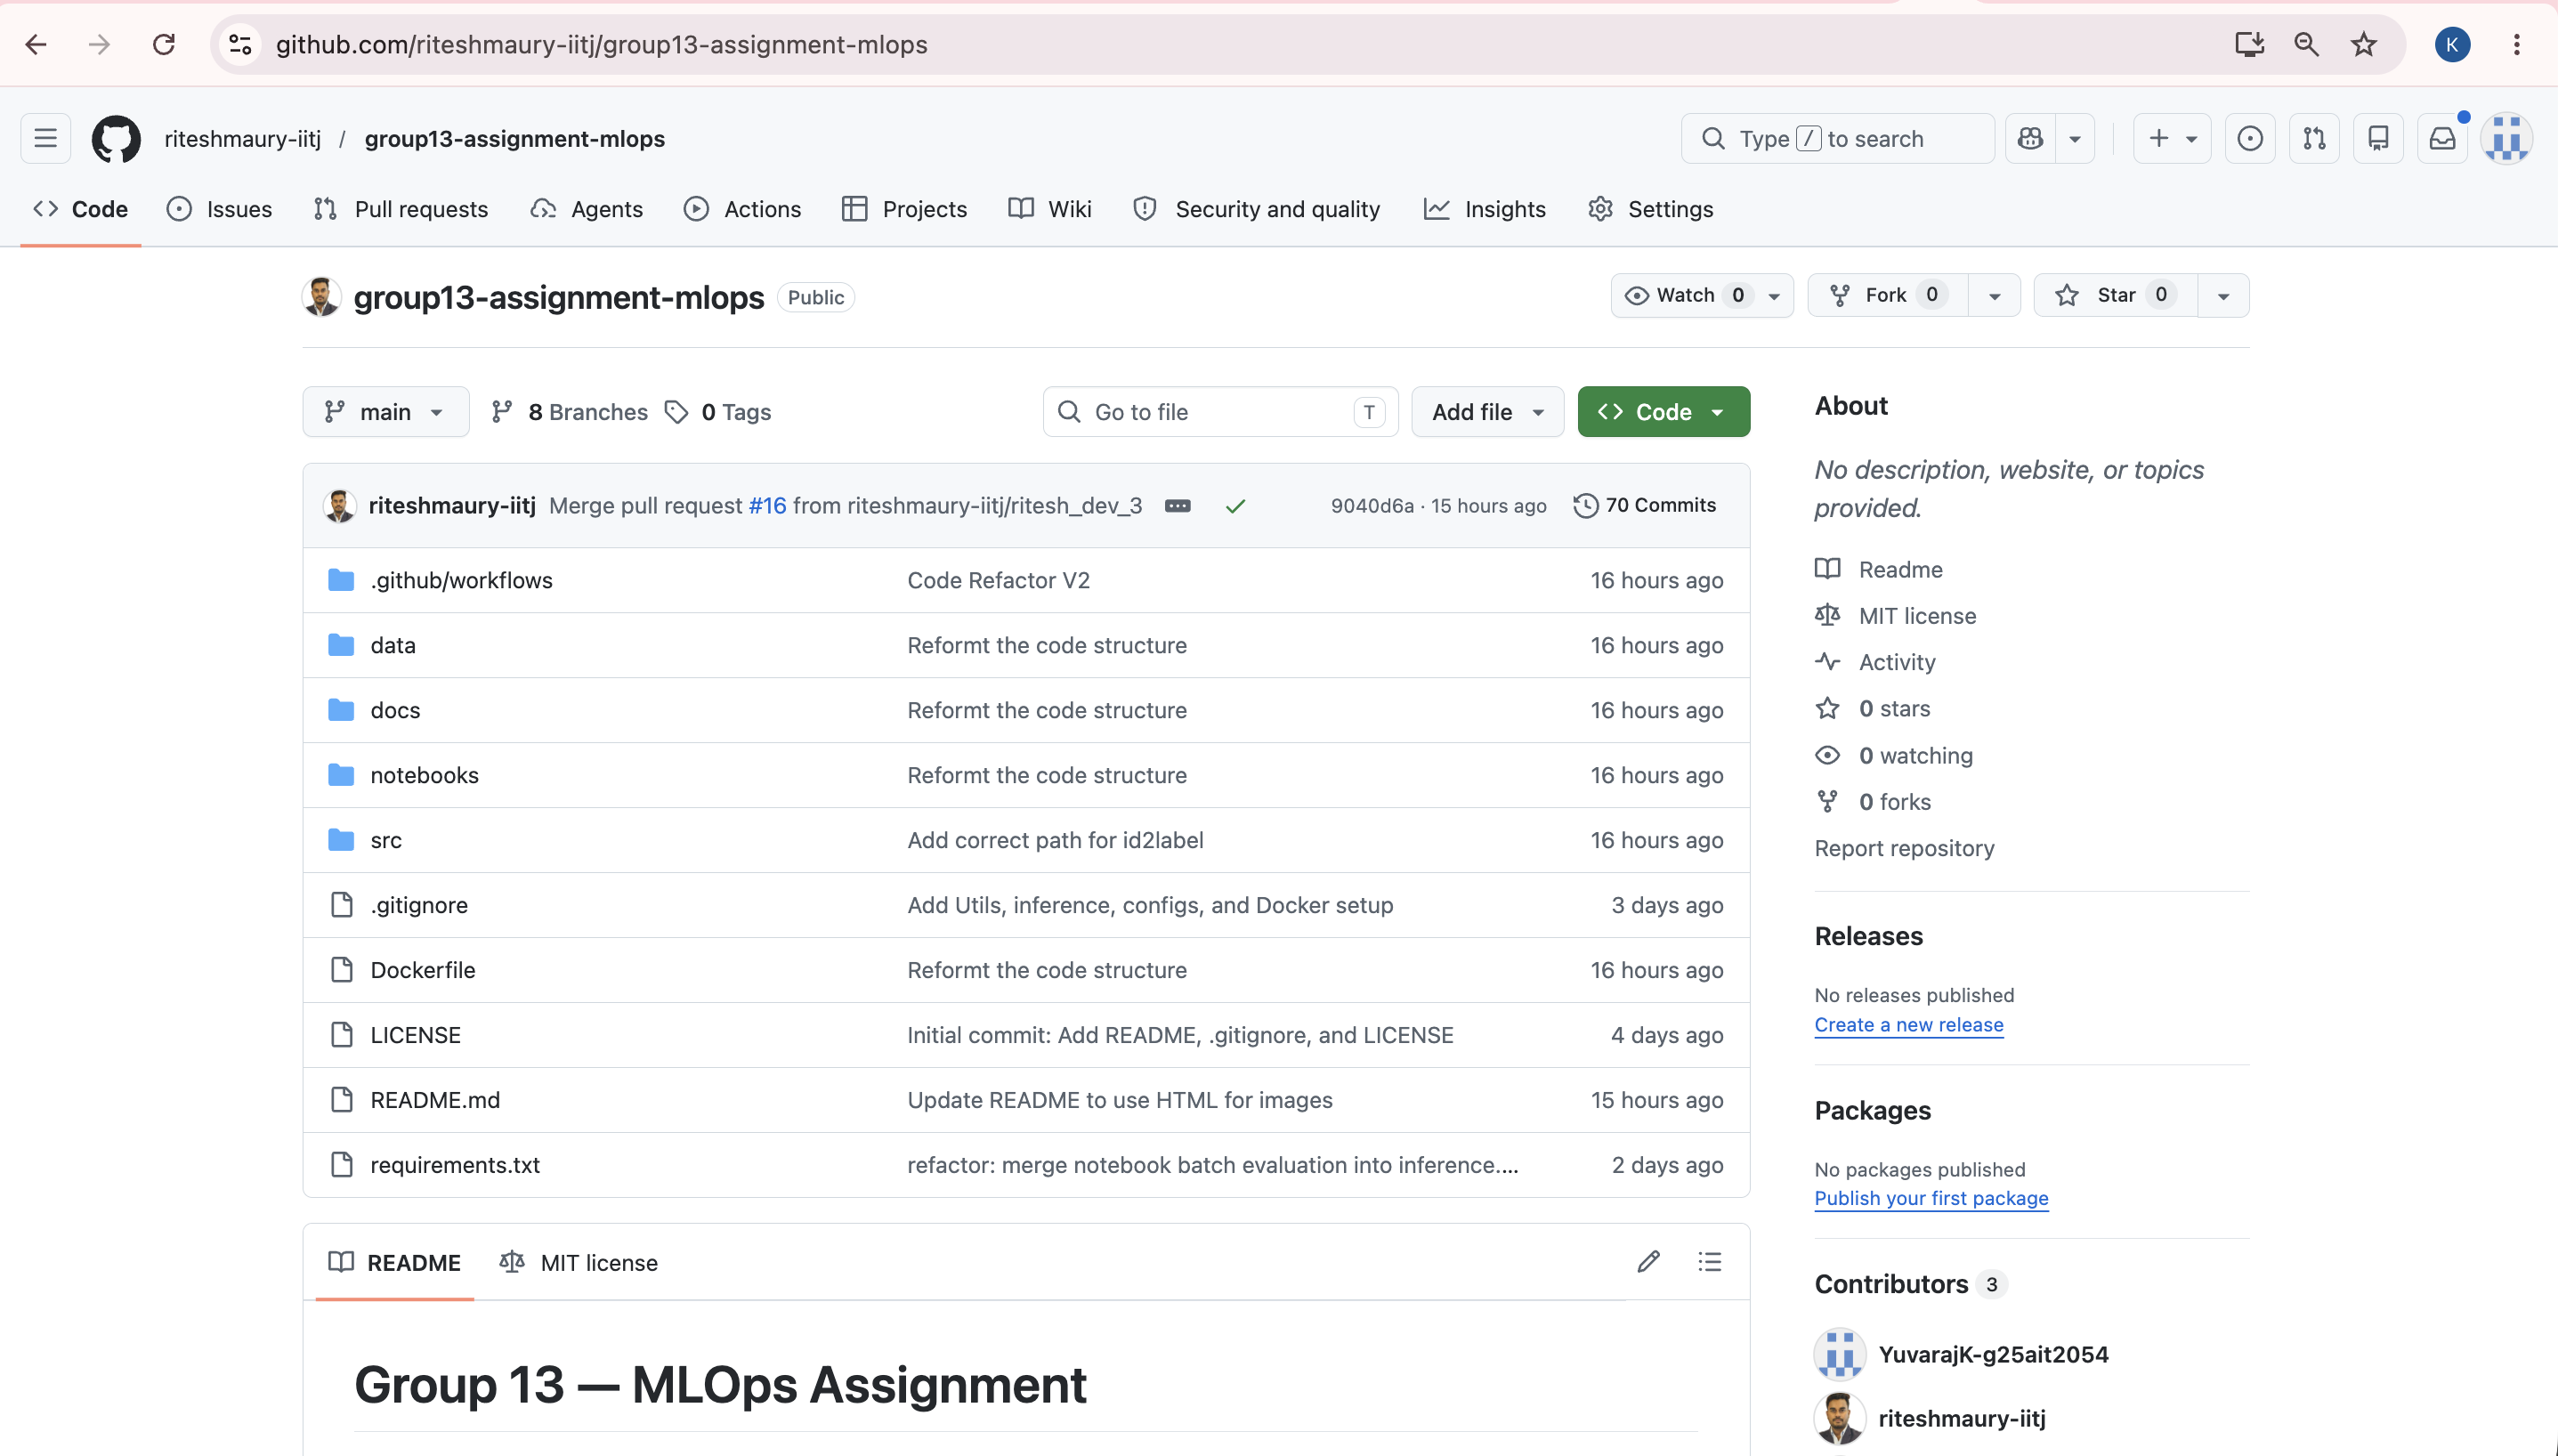
\includegraphics[width=0.85\textwidth]{screenshots/git_public_link.png}
\caption{GitHub repository --- public visibility and branch list}
\end{figure}

\begin{figure}[H]
\centering
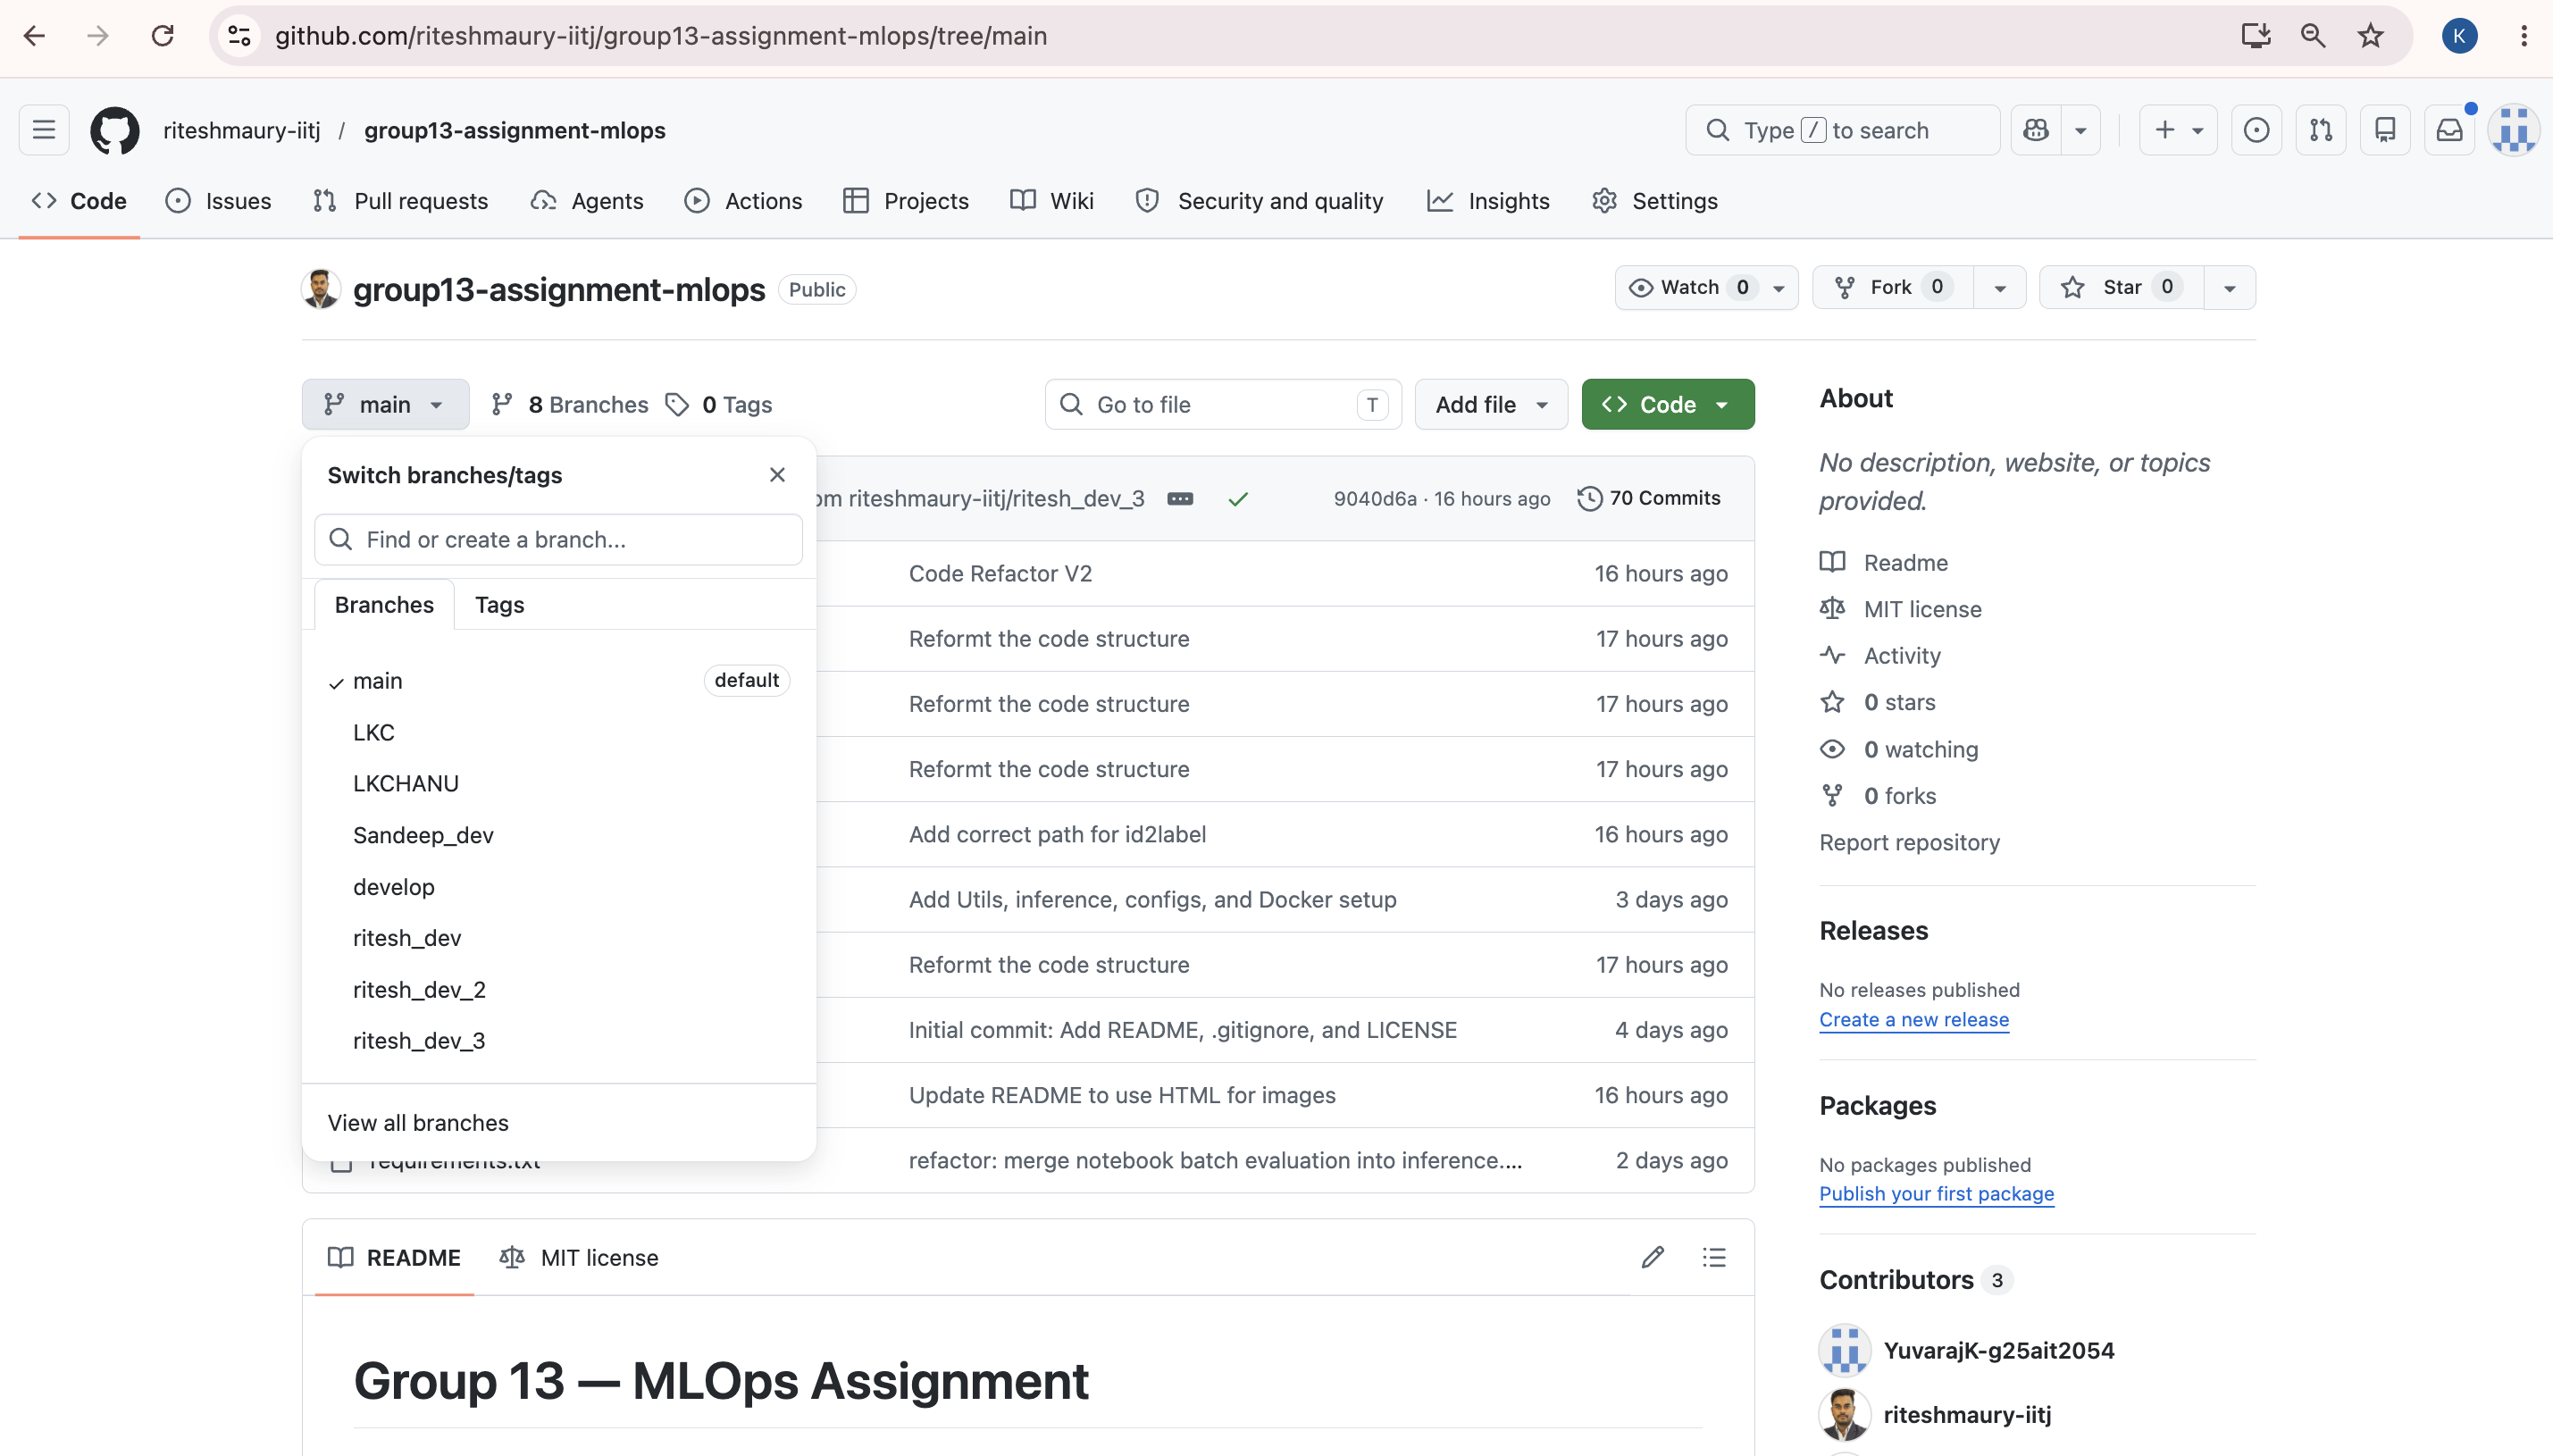
\includegraphics[width=0.85\textwidth]{screenshots/git_repo_details.png}
\caption{GitHub Settings --- Branch protection rule and repo details}
\end{figure}

\begin{figure}[H]
\centering
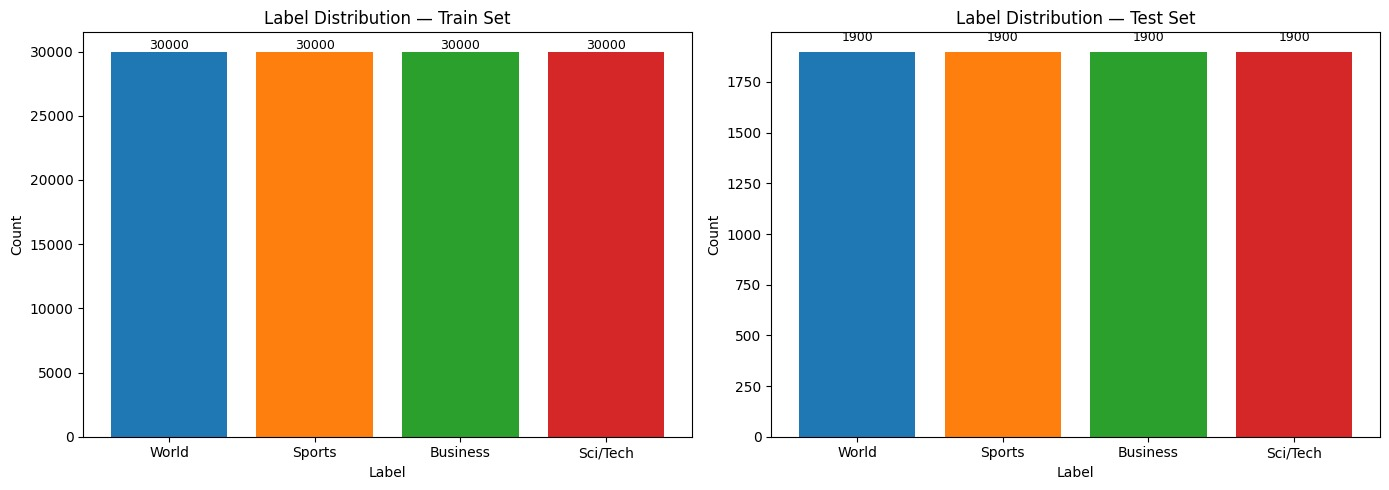
\includegraphics[width=0.85\textwidth]{screenshots/whatsapp_1.jpeg}
\caption{GitHub Settings --- Collaborators showing team members}
\end{figure}

\subsection{Task 2 --- Data Preparation \& Normalisation [15 marks]}

Dataset: \texttt{ag\_news} from HuggingFace (120,000 train / 7,600 test, 4 balanced classes). Preprocessing applied in \texttt{prepare\_data.ipynb}:
\begin{itemize}[noitemsep]
  \item Lowercase, remove URLs, strip HTML tags, remove punctuation, normalize whitespace.
  \item Label mapping saved to \texttt{id2label.json}: \texttt{\{0: World, 1: Sports, 2: Business, 3: Sci/Tech\}}.
  \item Tokenized with \texttt{max\_length=128}.
\end{itemize}

\subsection{Task 3 --- Model Selection [10 marks]}

Selected \textbf{distilbert-base-uncased}: 66M parameters, retains $\sim$97\% of BERT performance, and trains on AG News in $\sim$40 min on a T4 GPU. Loaded via \texttt{AutoModelForSequenceClassification} with \texttt{num\_labels=4} and \texttt{id2label}/\texttt{label2id} mappings. Tokenizer uses \texttt{truncation=True}, \texttt{padding=True}, \texttt{max\_length=128}.

% ======================== PAGE 3 ========================
\section{Training, W\&B Tracking and HuggingFace Deployment (Tasks 4--5)}

\subsection{Task 4 --- Training on Kaggle with W\&B [25 marks]}

Training on Kaggle (GPU T4 \texttimes 2), tracked via W\&B project \texttt{mlops-assignment3}. Secrets (W\&B, HuggingFace, GitHub) stored as Kaggle Secrets, loaded via \texttt{UserSecretsClient}.

\vspace{0.3cm}
\textbf{Hyperparameter Comparison:}

\renewcommand{\arraystretch}{1.4}
\begin{tabular}{lcc}
\toprule
\textbf{Hyperparameter}   & \textbf{Version 1 (run-v1)} & \textbf{Version 2 (run-v2)} \\
\midrule
Base Model                & distilbert-base-uncased     & distilbert-base-uncased \\
Learning Rate             & 2e-5                        & 5e-5                    \\
Batch Size (train)        & 16                          & 64                      \\
Epochs                    & 3                           & 5                       \\
Weight Decay              & 0.01                        & 0.01                    \\
Max Sequence Length       & 128                         & 128                     \\
Evaluation Strategy       & Per epoch                   & Per epoch               \\
Best Model Metric         & F1 (weighted)               & F1 (weighted)           \\
\bottomrule
\end{tabular}

\vspace{0.4cm}
\textbf{Results:}

\renewcommand{\arraystretch}{1.4}
\begin{tabular}{lccc}
\toprule
\textbf{Version} & \textbf{Accuracy} & \textbf{F1 (weighted)} & \textbf{Eval Loss} \\
\midrule
Version 1 (run-v1) & \textbf{94.34\%} & \textbf{0.9434} & 0.3679 \\
Version 2 (run-v2) & 94.12\%          & 0.9412          & 0.3575 \\
\bottomrule
\end{tabular}

\vspace{0.4cm}
Version 1 achieved higher accuracy and F1; selected as the final model. Both versions exceeded 94\% accuracy.

\begin{figure}[H]
\centering
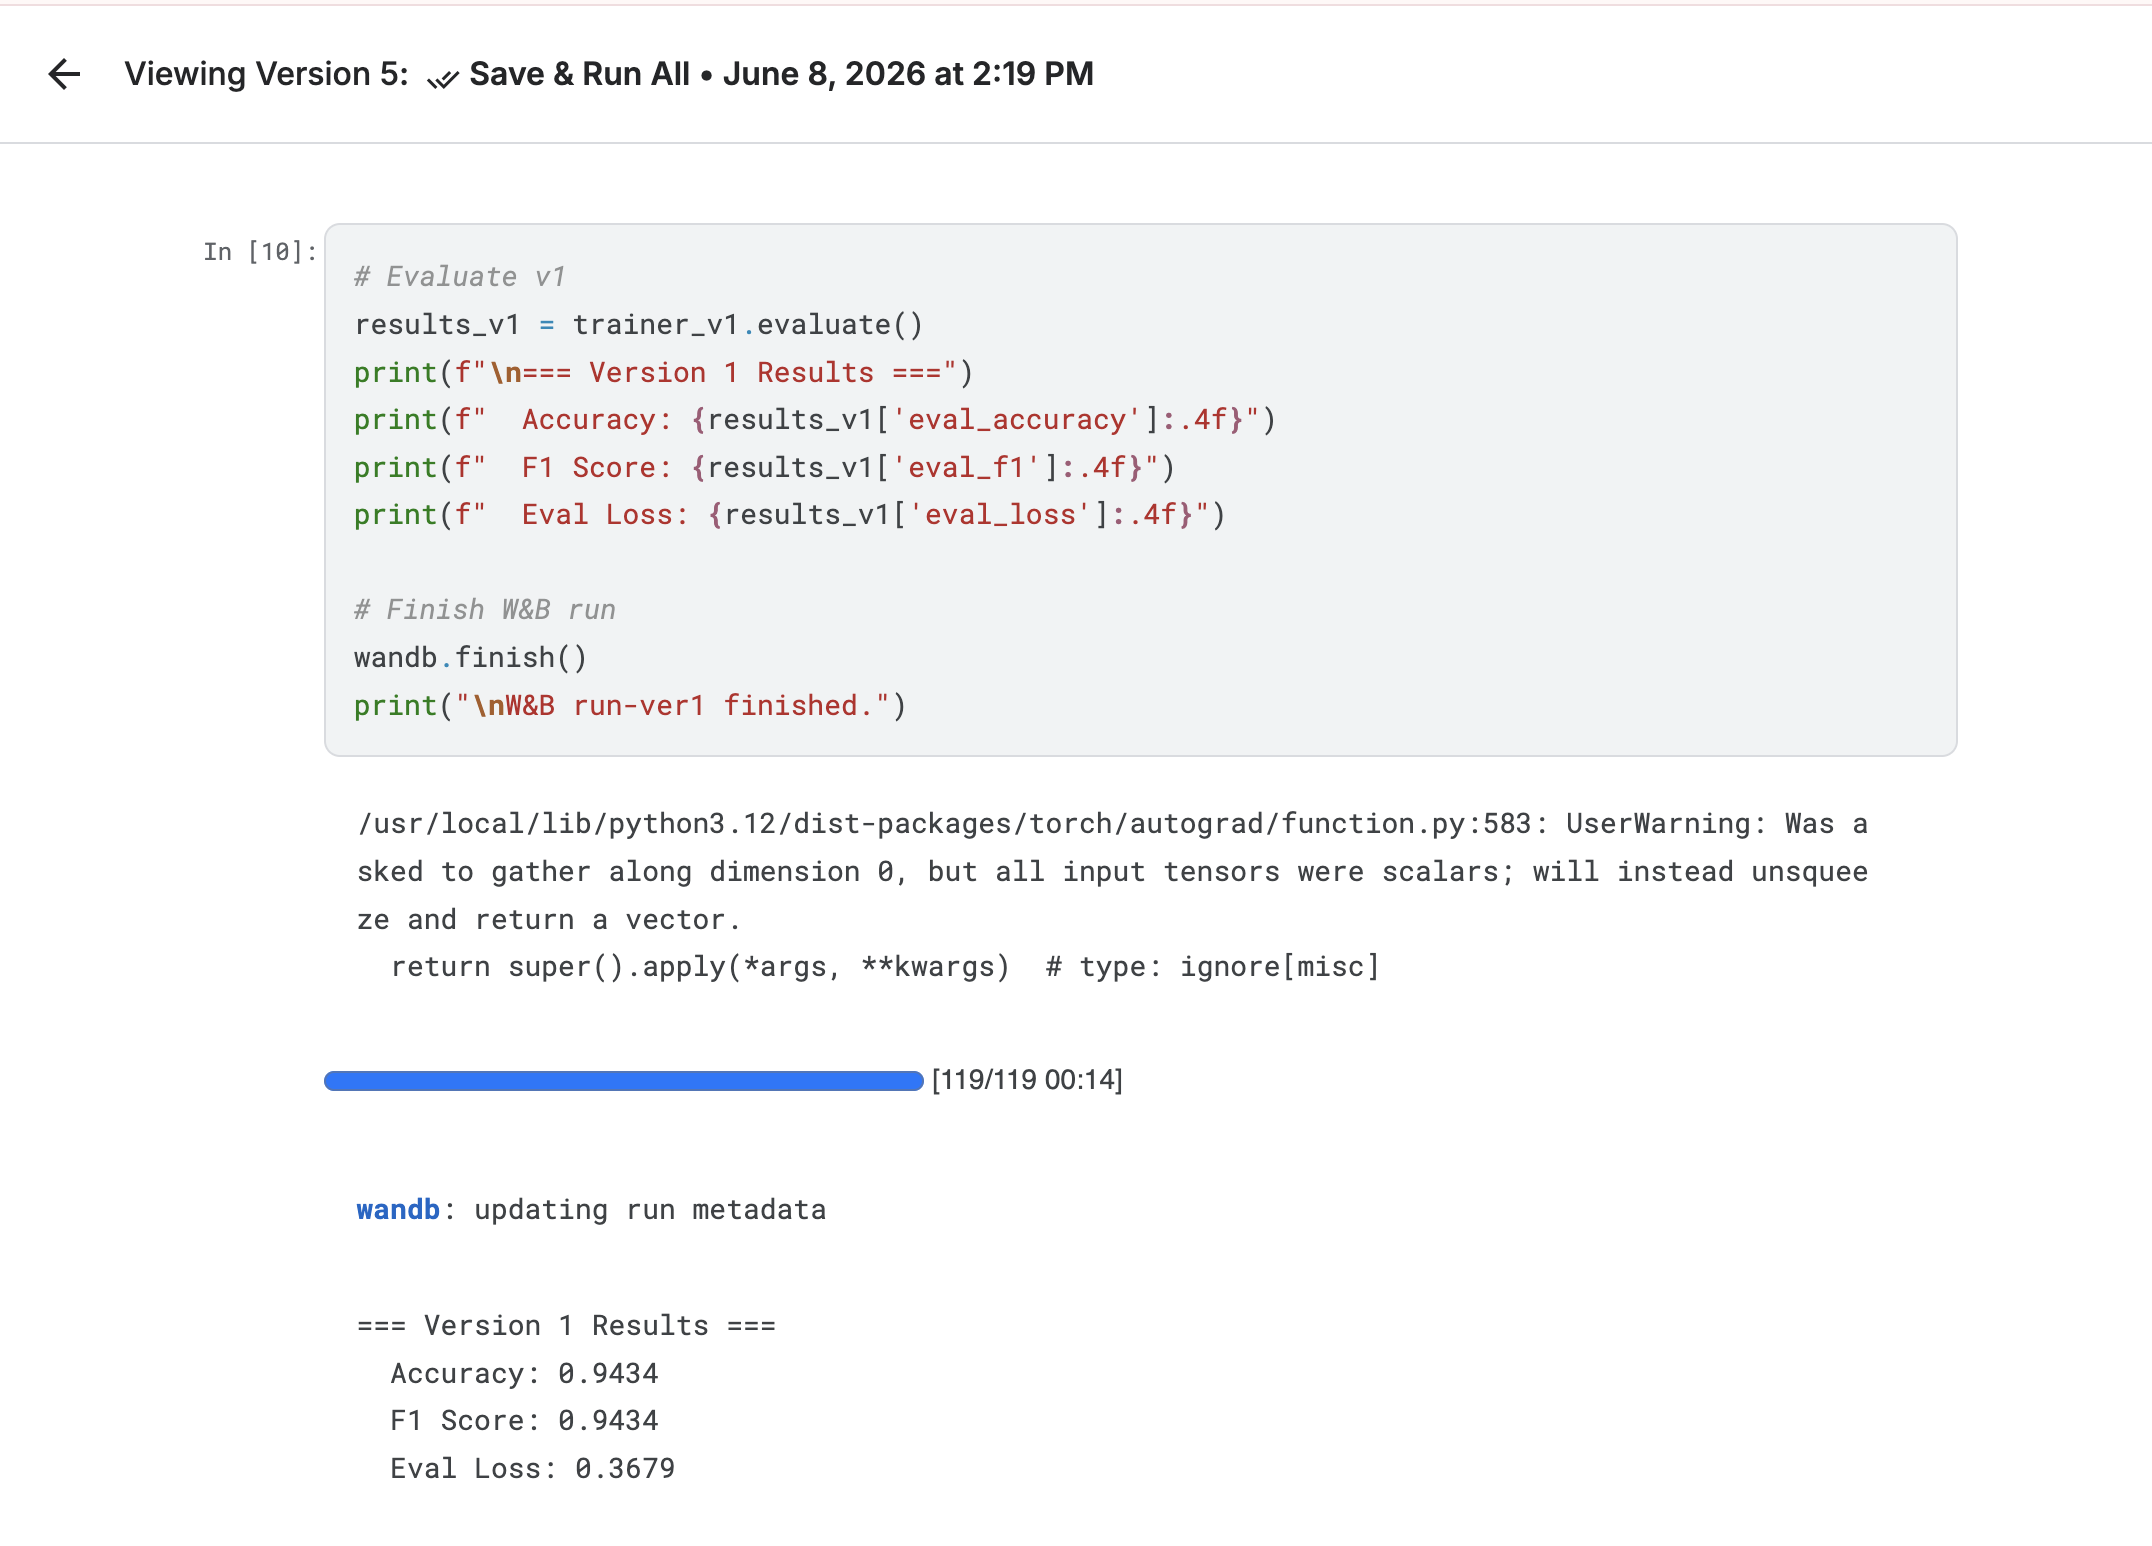
\includegraphics[width=0.85\textwidth]{screenshots/kaggle_V1.png}
\caption{Kaggle notebook --- Version 1 training output (eval accuracy 94.34\%, F1 0.9434)}
\end{figure}

\begin{figure}[H]
\centering
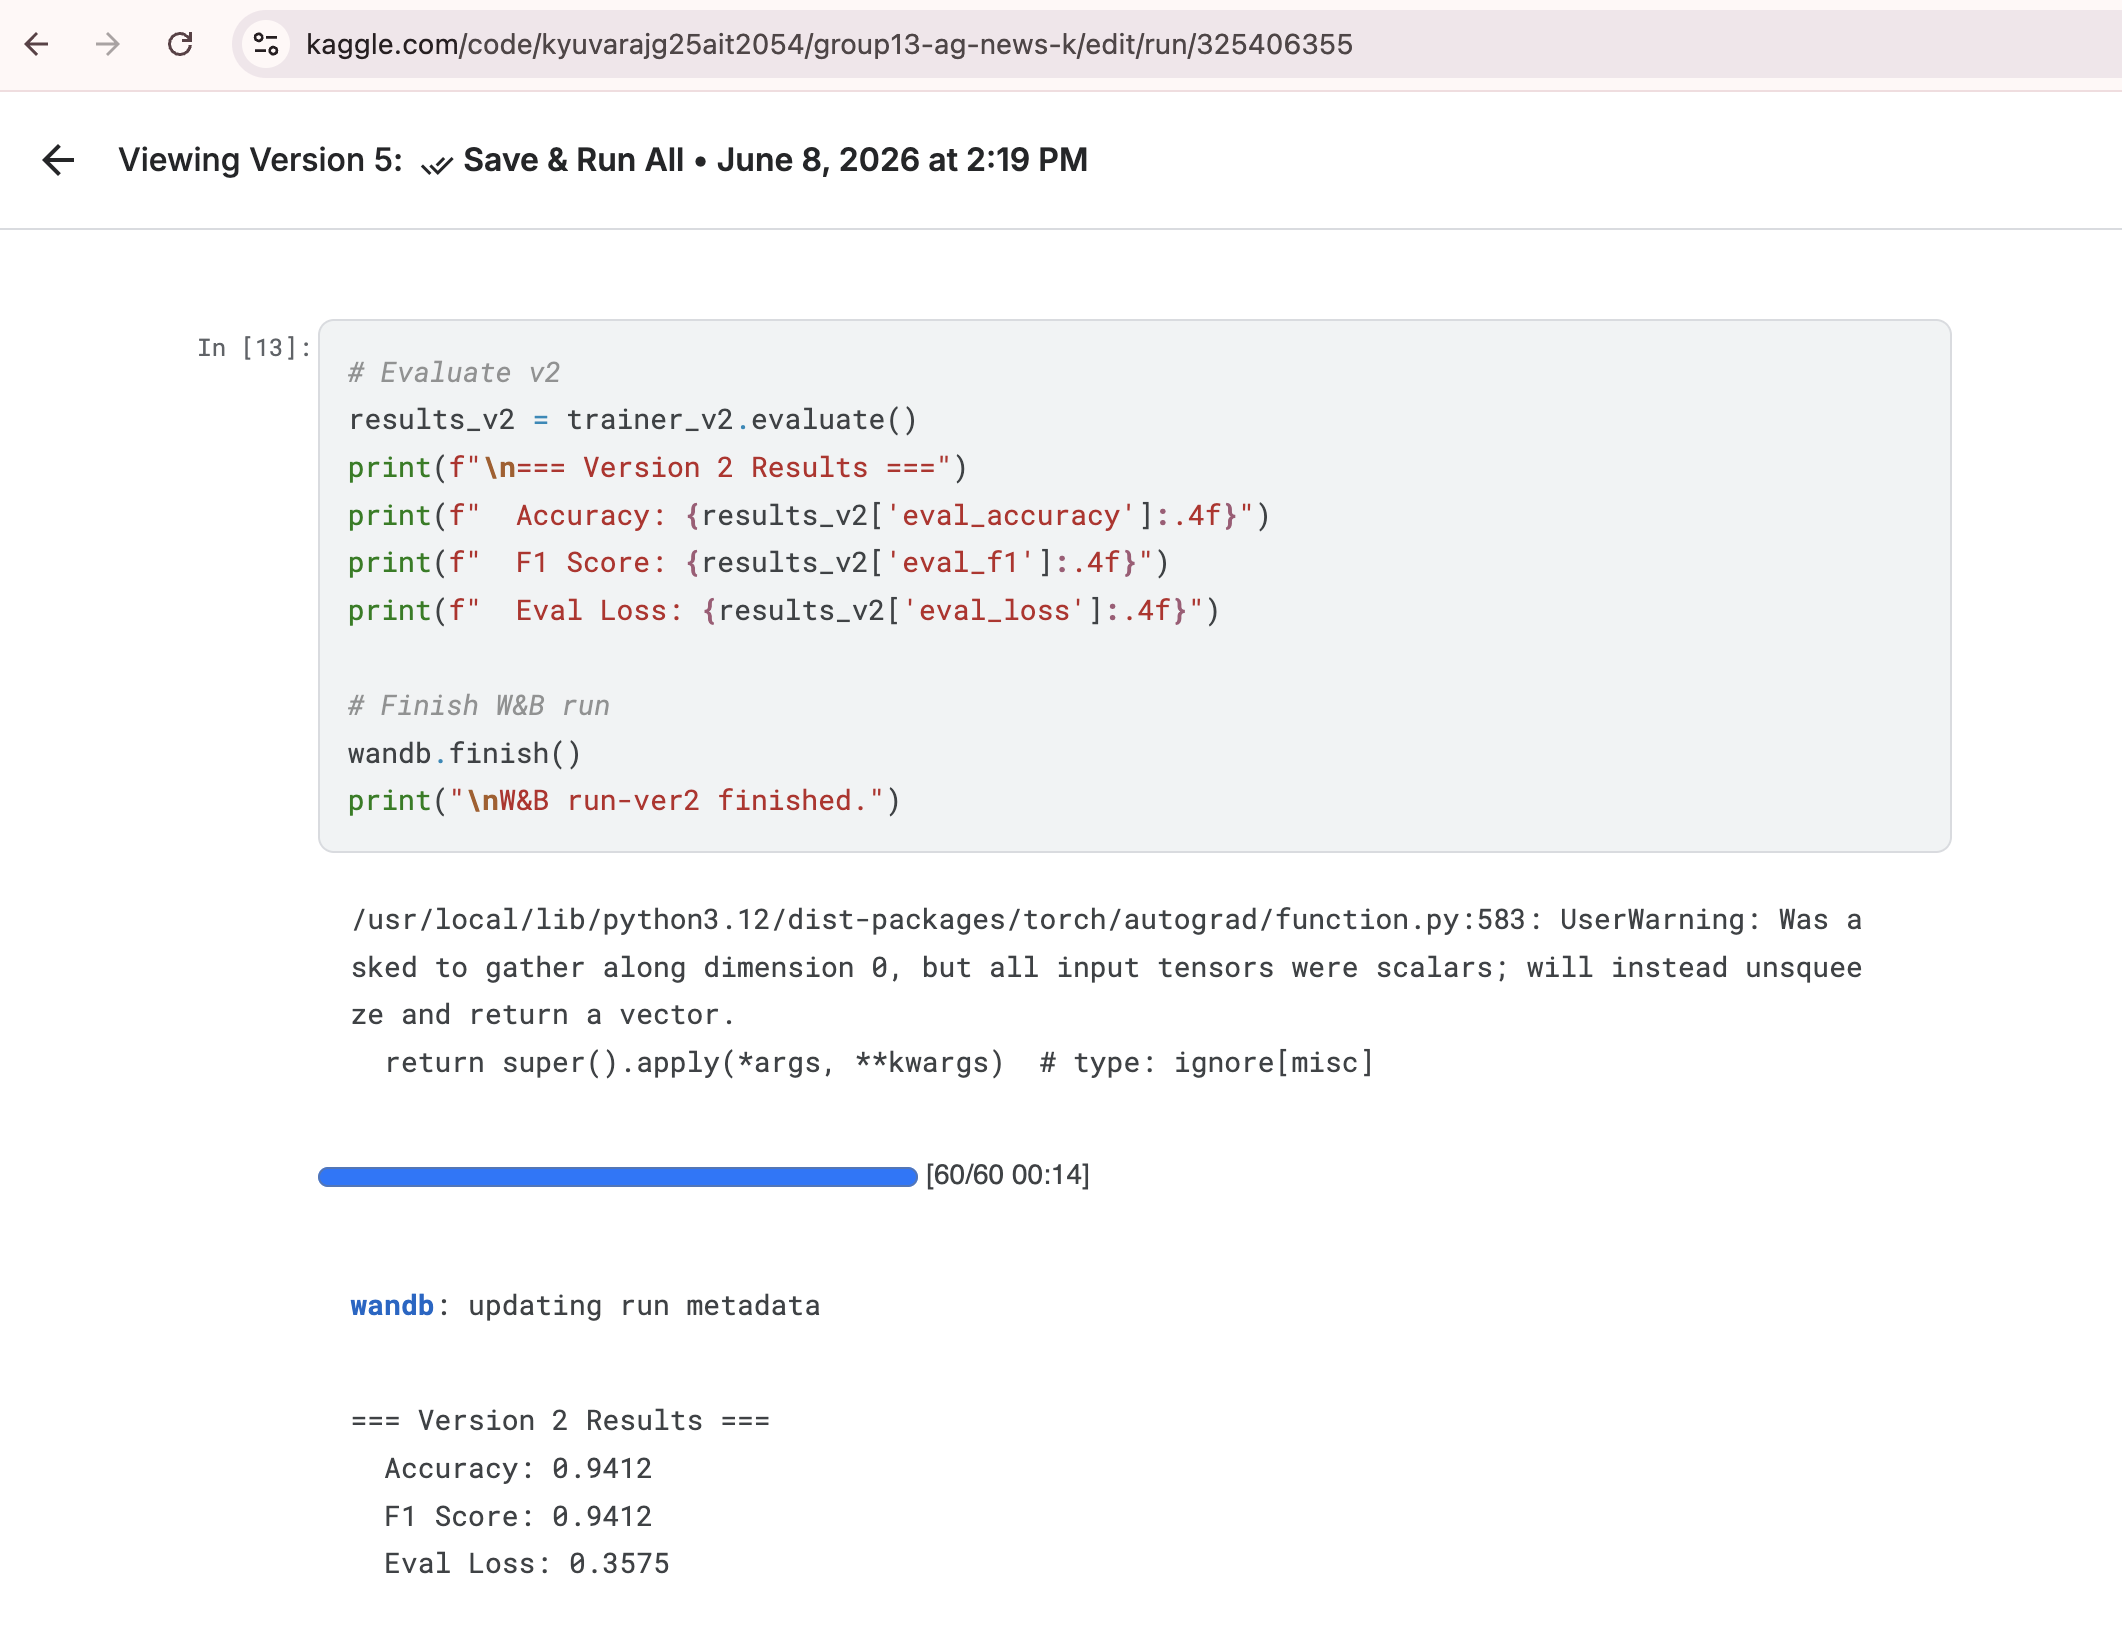
\includegraphics[width=0.85\textwidth]{screenshots/kaggle_V2.png}
\caption{Kaggle notebook --- Version 2 training output (eval accuracy 94.12\%, F1 0.9412)}
\end{figure}

\begin{figure}[H]
\centering
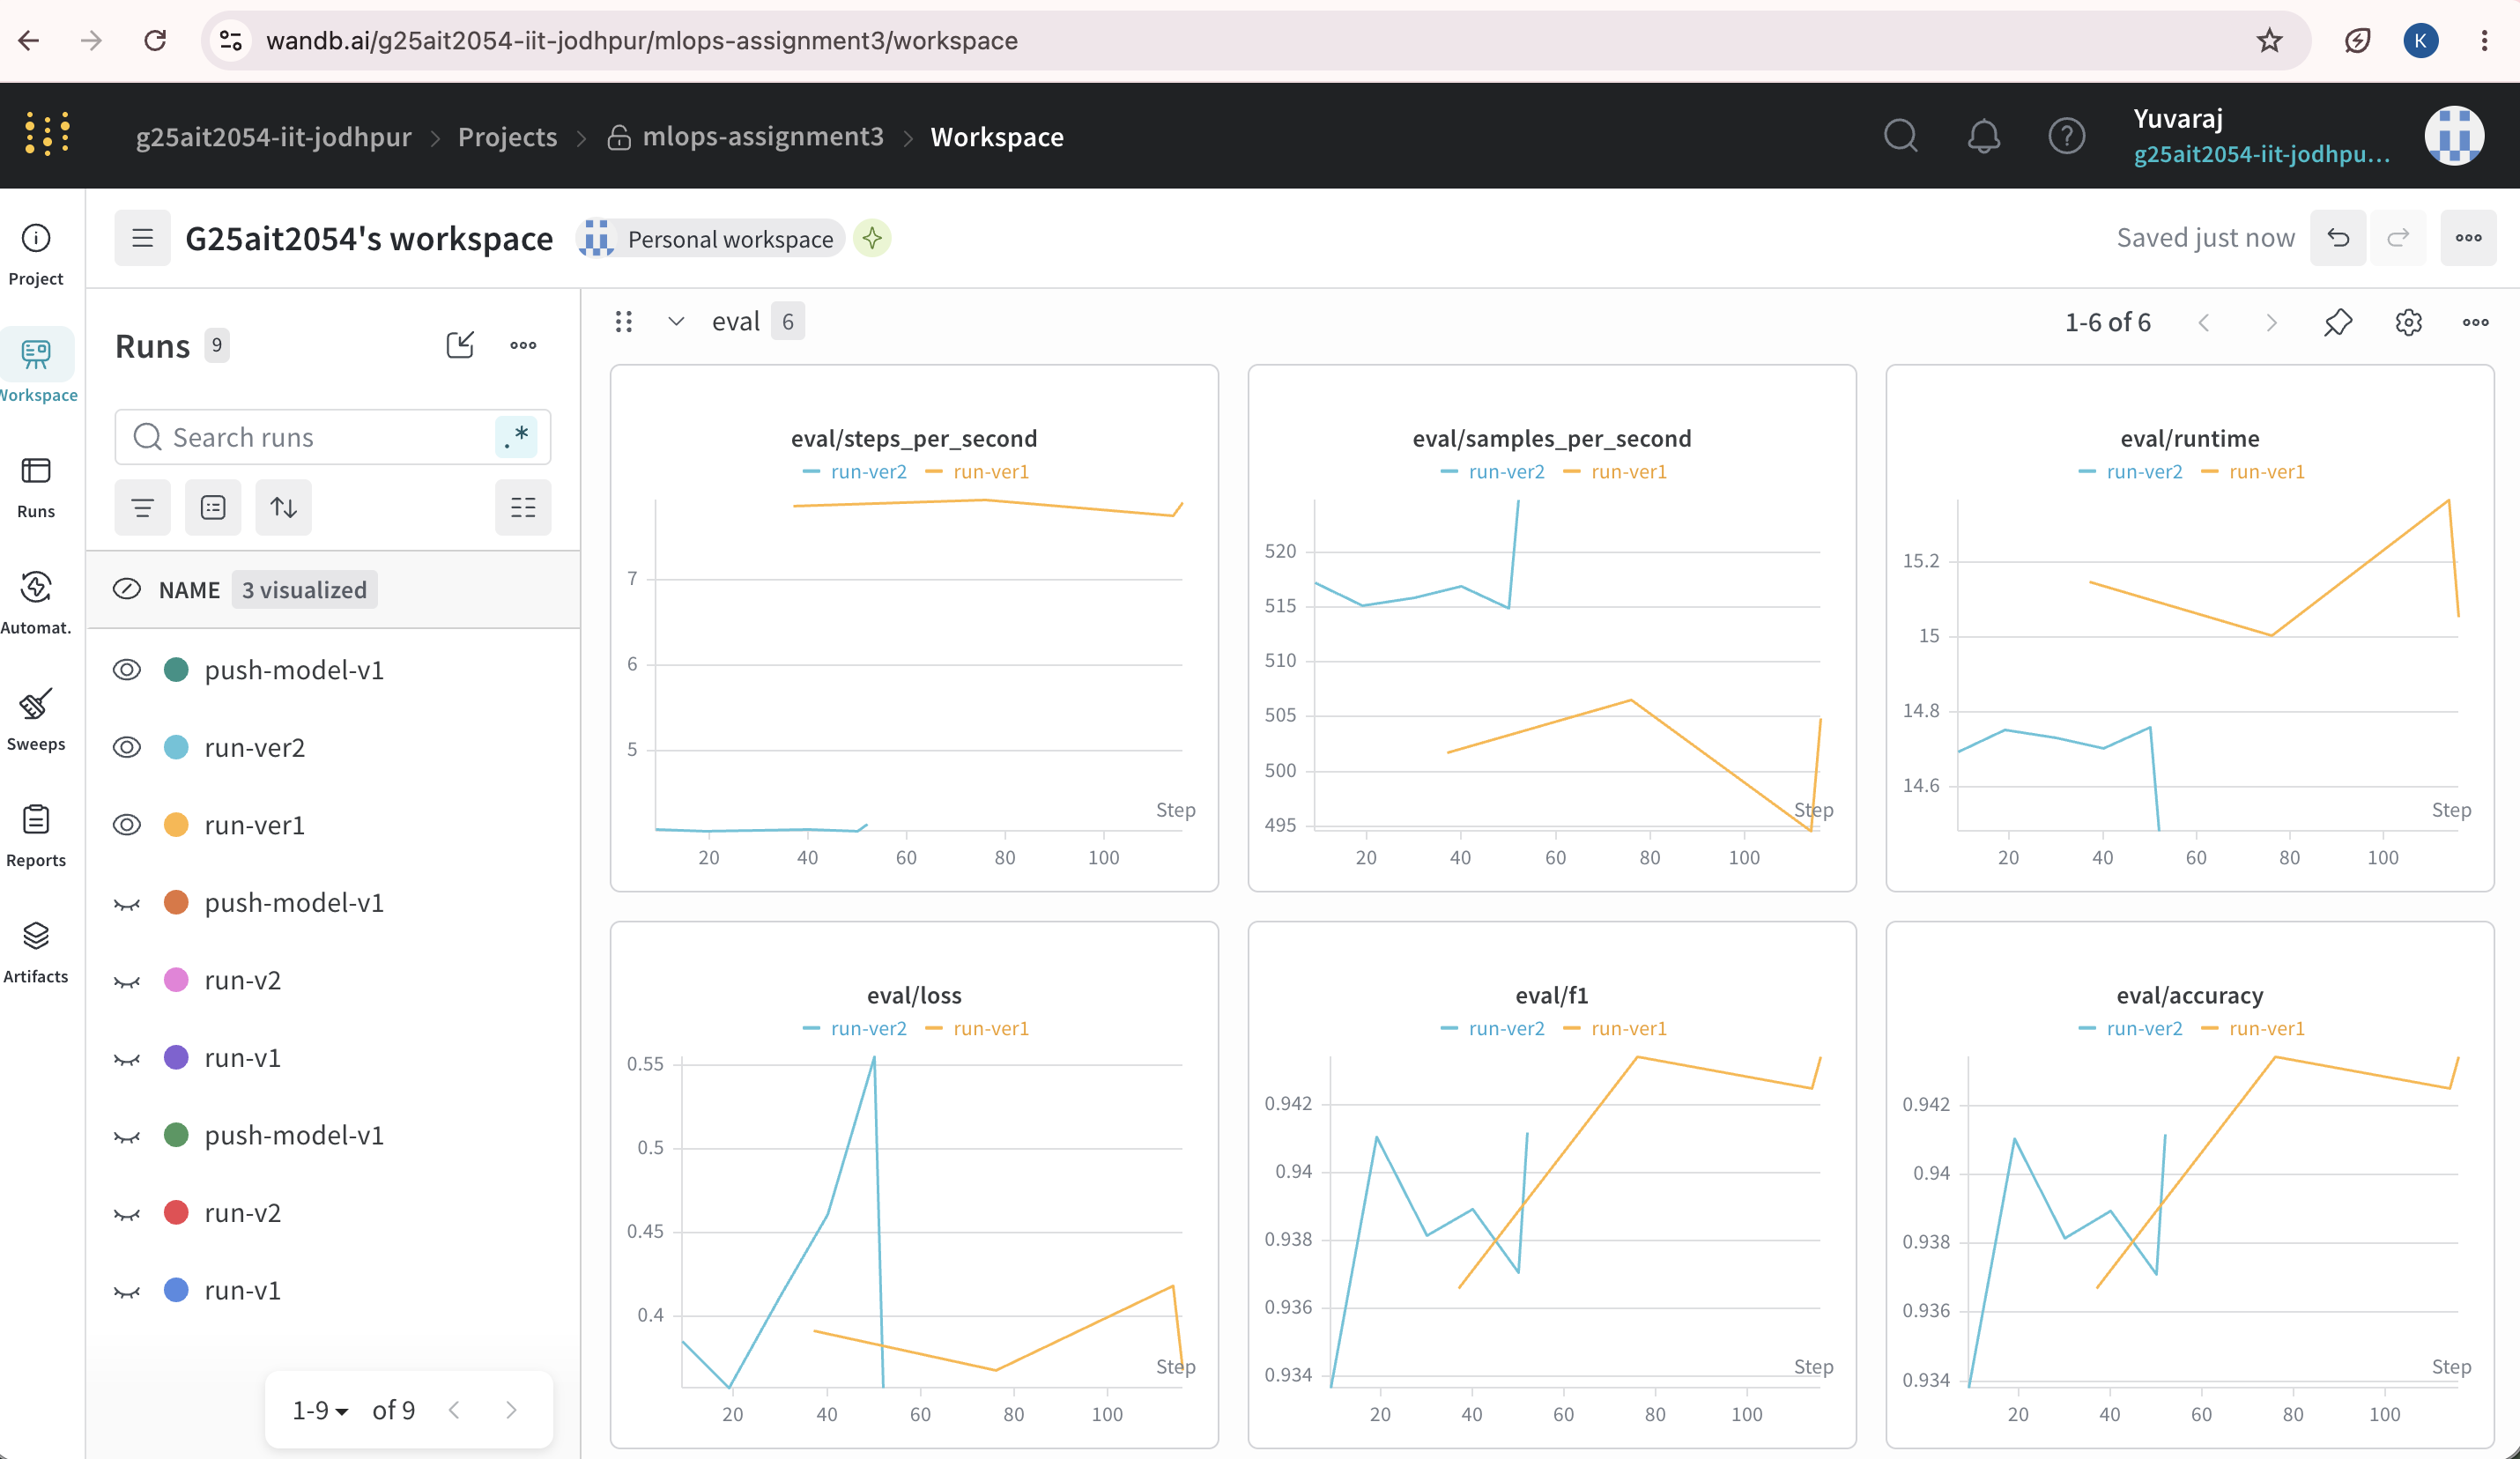
\includegraphics[width=0.85\textwidth]{screenshots/wandb_Eval.png}
\caption{W\&B dashboard --- mlops-assignment3 showing run-v1 and run-v2 with metrics}
\end{figure}

\begin{figure}[H]
\centering
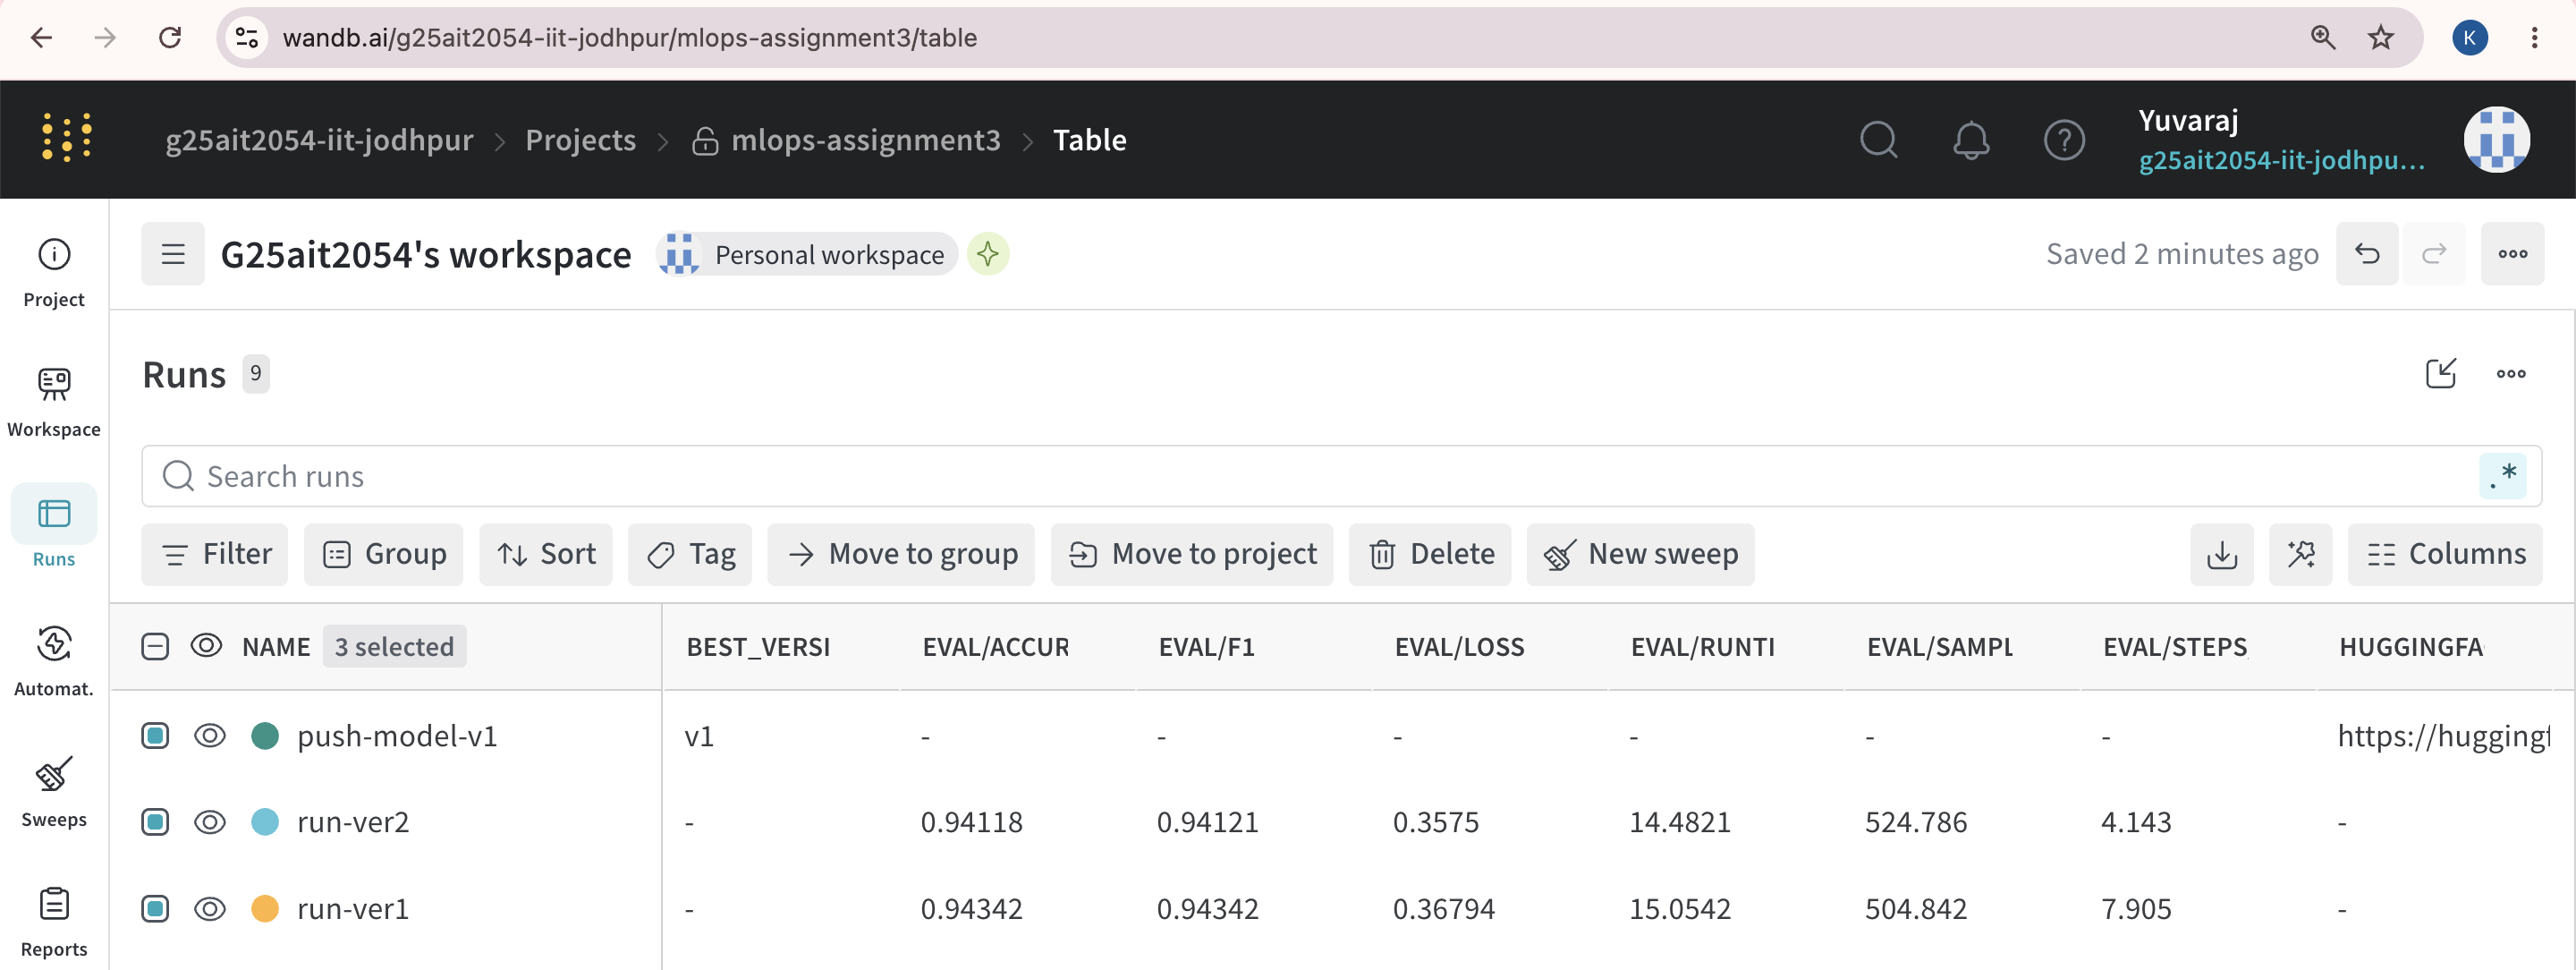
\includegraphics[width=0.85\textwidth]{screenshots/wandb_compare.png}
\caption{W\&B comparison chart --- eval/accuracy and eval/loss across both runs}
\end{figure}

\subsection{Task 5 --- Push Model to HuggingFace Hub [5 marks]}

Version 1 pushed to HuggingFace Hub via \texttt{trainer.push\_to\_hub()}. Model is public at:
\begin{center}
\href{https://huggingface.co/YuvarajK-g25ait2054/ag-news-distilbert}{\texttt{https://huggingface.co/YuvarajK-g25ait2054/ag-news-distilbert}}
\end{center}
Model card (\texttt{MODEL\_CARD.md}) covers description, hyperparameters, evaluation results, and usage.

\begin{figure}[H]
\centering
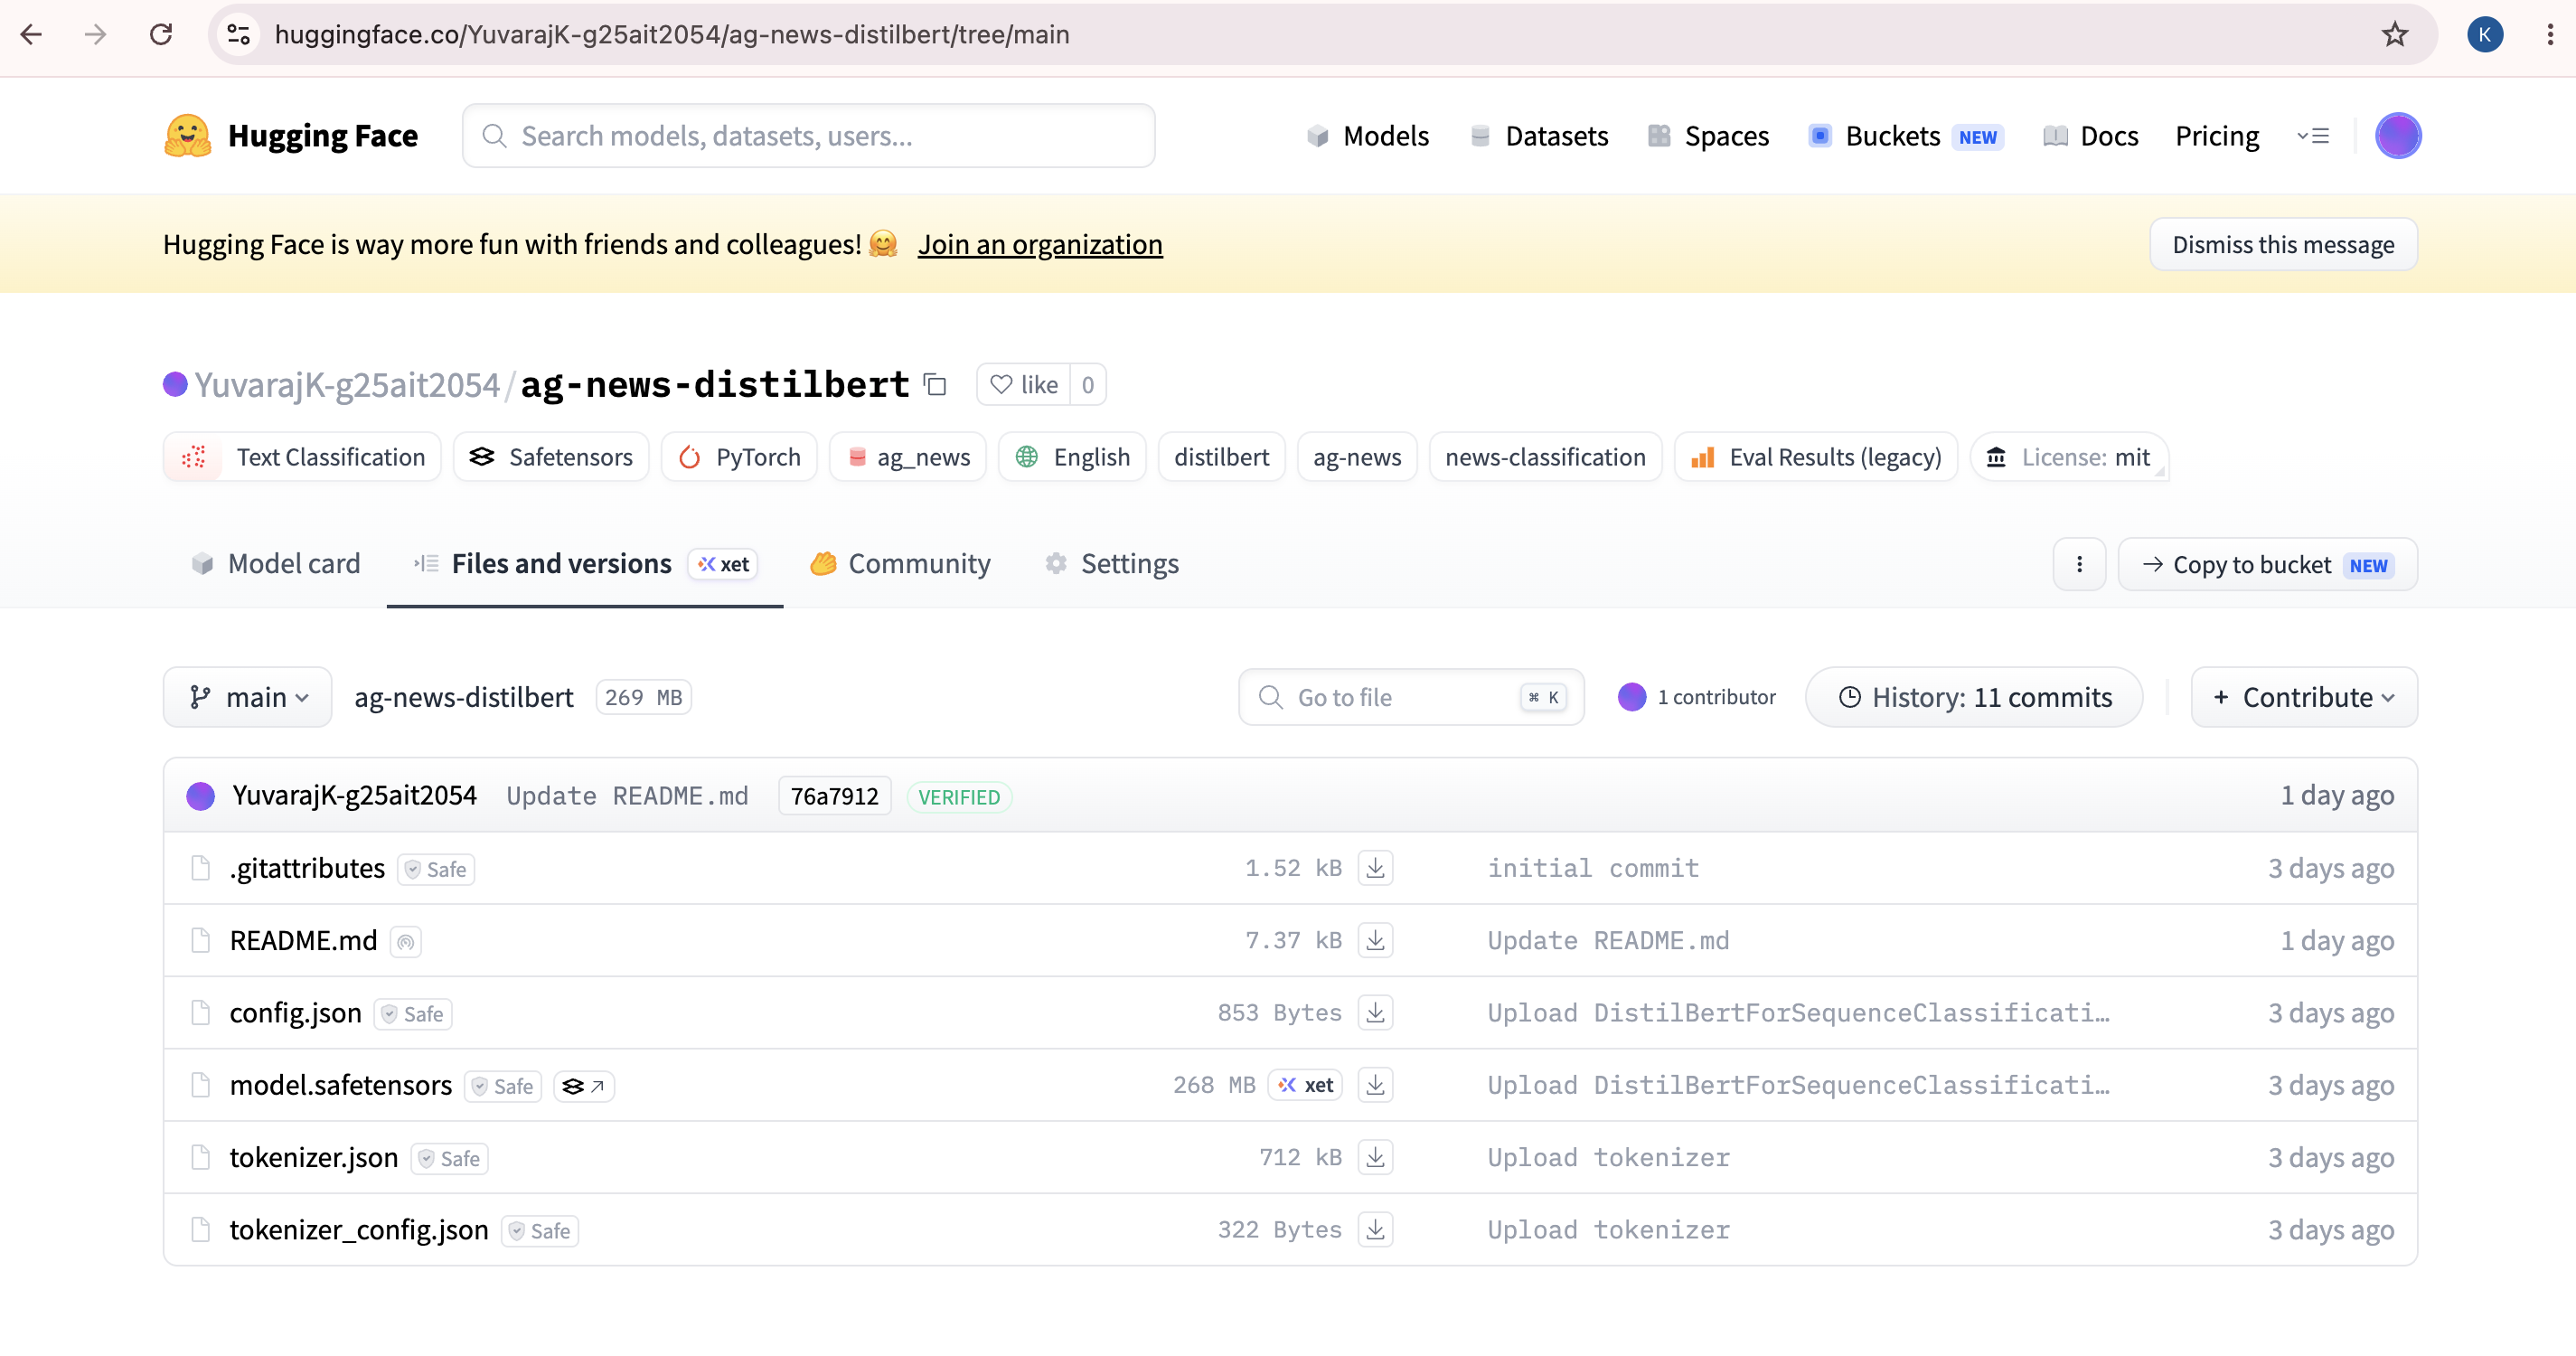
\includegraphics[width=0.85\textwidth]{screenshots/Huggingface.png}
\caption{HuggingFace model page --- YuvarajK-g25ait2054/ag-news-distilbert}
\end{figure}

% ======================== PAGE 4 ========================
\section{Docker Deployment and GitHub Actions CI/CD (Tasks 6--7)}

\subsection{Task 6 --- Dockerfile [10 marks]}

Docker image hosted at \href{https://hub.docker.com/r/yuvarajkg25ait2054/ag-news-classifier}{\texttt{yuvarajkg25ait2054/ag-news-classifier:latest}}.

\begin{itemize}[noitemsep]
  \item Base: \texttt{python:3.10-slim}; PyTorch \texttt{2.5.1+cpu} from PyTorch's CPU wheel index.
  \item Model pre-baked into image during \texttt{docker build} --- no internet required at runtime.
  \item Default \texttt{CMD} runs \texttt{--demo} mode: classifies all 4 sample texts from \texttt{inference.ipynb} Cell~7.
\end{itemize}

\begin{verbatim}
# Demo mode (default) -- runs all 4 notebook texts:
docker run --rm yuvarajkg25ait2054/ag-news-classifier:latest

# Single text:
docker run --rm yuvarajkg25ait2054/ag-news-classifier:latest \
  --text "Stock market rises on strong earnings"
\end{verbatim}

\begin{figure}[H]
\centering
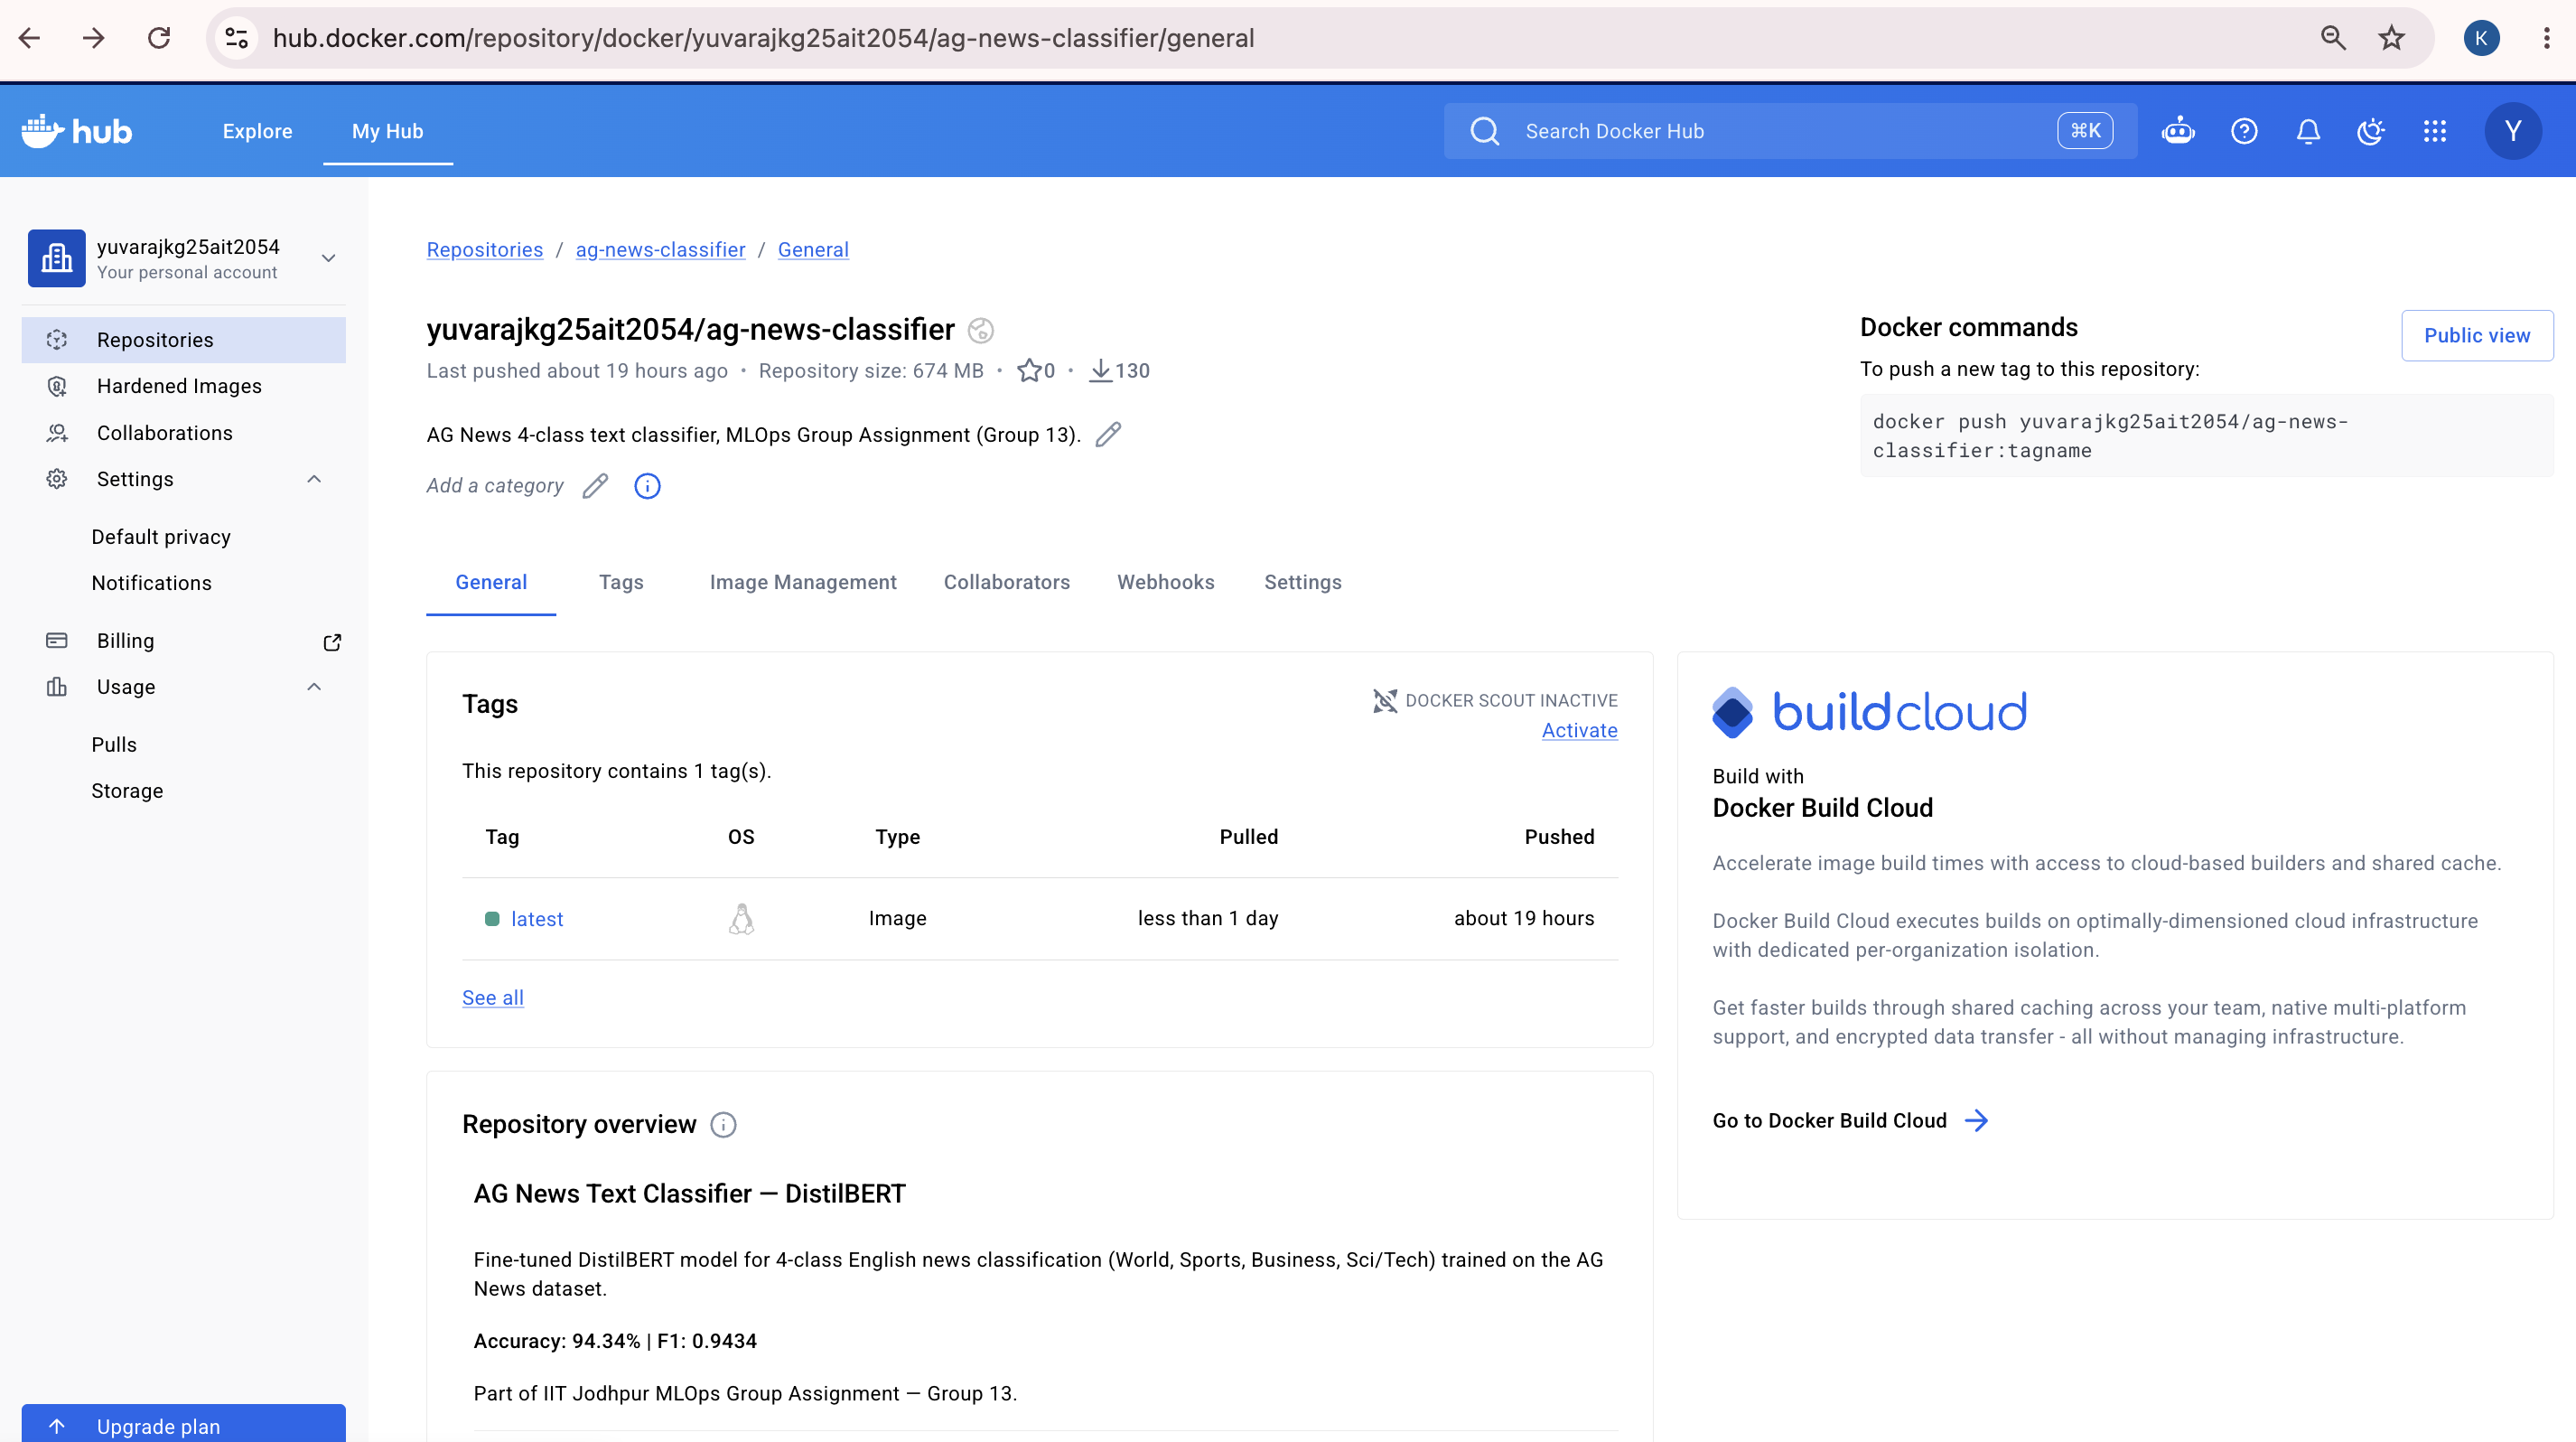
\includegraphics[width=0.85\textwidth]{screenshots/Docker_public.png}
\caption{Docker Hub --- yuvarajkg25ait2054/ag-news-classifier (publicly pullable)}
\end{figure}

\begin{figure}[H]
\centering
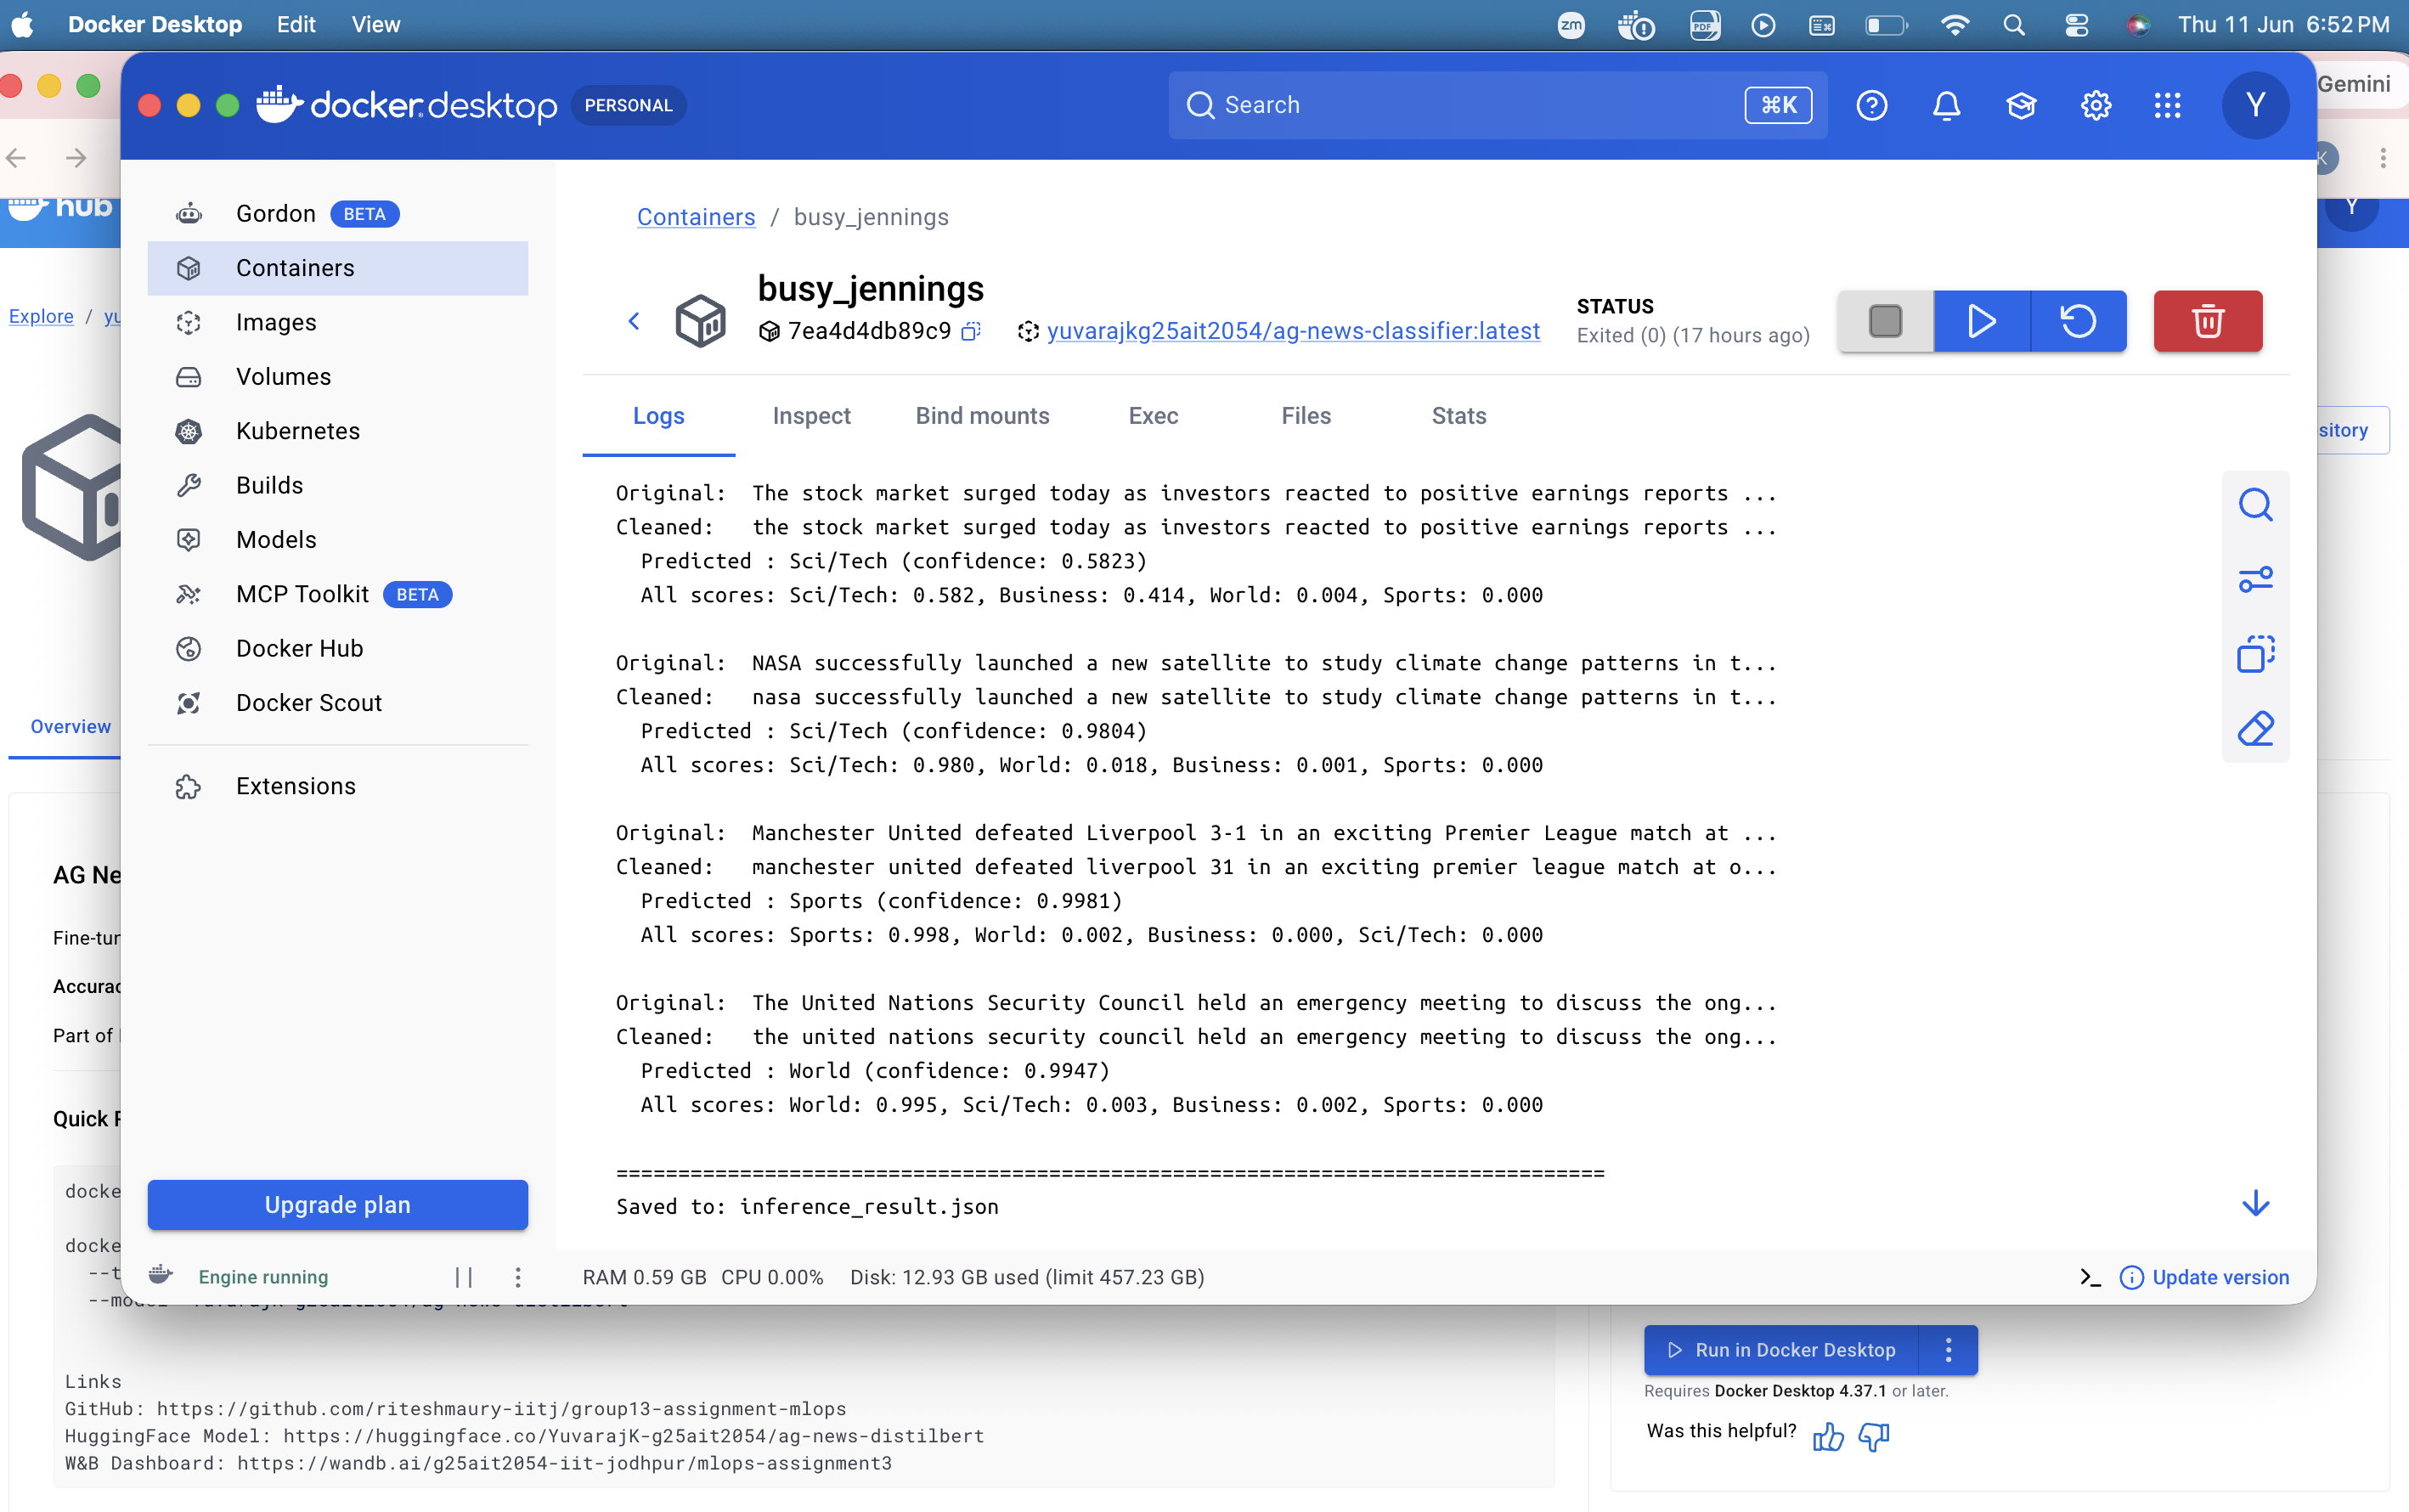
\includegraphics[width=0.85\textwidth]{screenshots/Docker_output.png}
\caption{Docker container --- demo mode classifying all 4 sample texts}
\end{figure}

\subsection{Task 7 --- GitHub Actions Workflows [15 marks]}

Two workflows under \texttt{.github/workflows/}:

\begin{itemize}[noitemsep]
  \item \textbf{ci.yml} --- triggered on push/PR to \texttt{develop} and \texttt{main}. Validates required files, runs Python syntax check (\texttt{py\_compile}), and validates JSON files.
  \item \textbf{inference.yml} --- installs dependencies and runs \texttt{inference.py} end-to-end with a hardcoded test sentence against the HuggingFace model.
\end{itemize}

Both workflows pass with green checkmarks.

\begin{figure}[H]
\centering
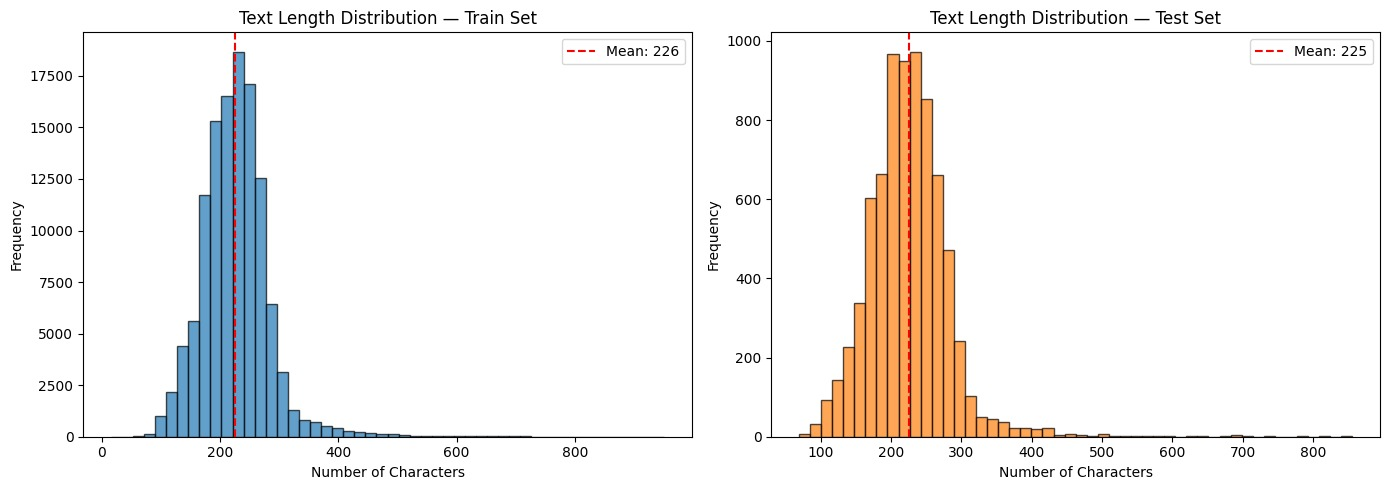
\includegraphics[width=0.85\textwidth]{screenshots/whatsapp_2.jpeg}
\caption{GitHub Actions --- CI Pipeline and Inference workflow with green checkmarks}
\end{figure}

\begin{figure}[H]
\centering
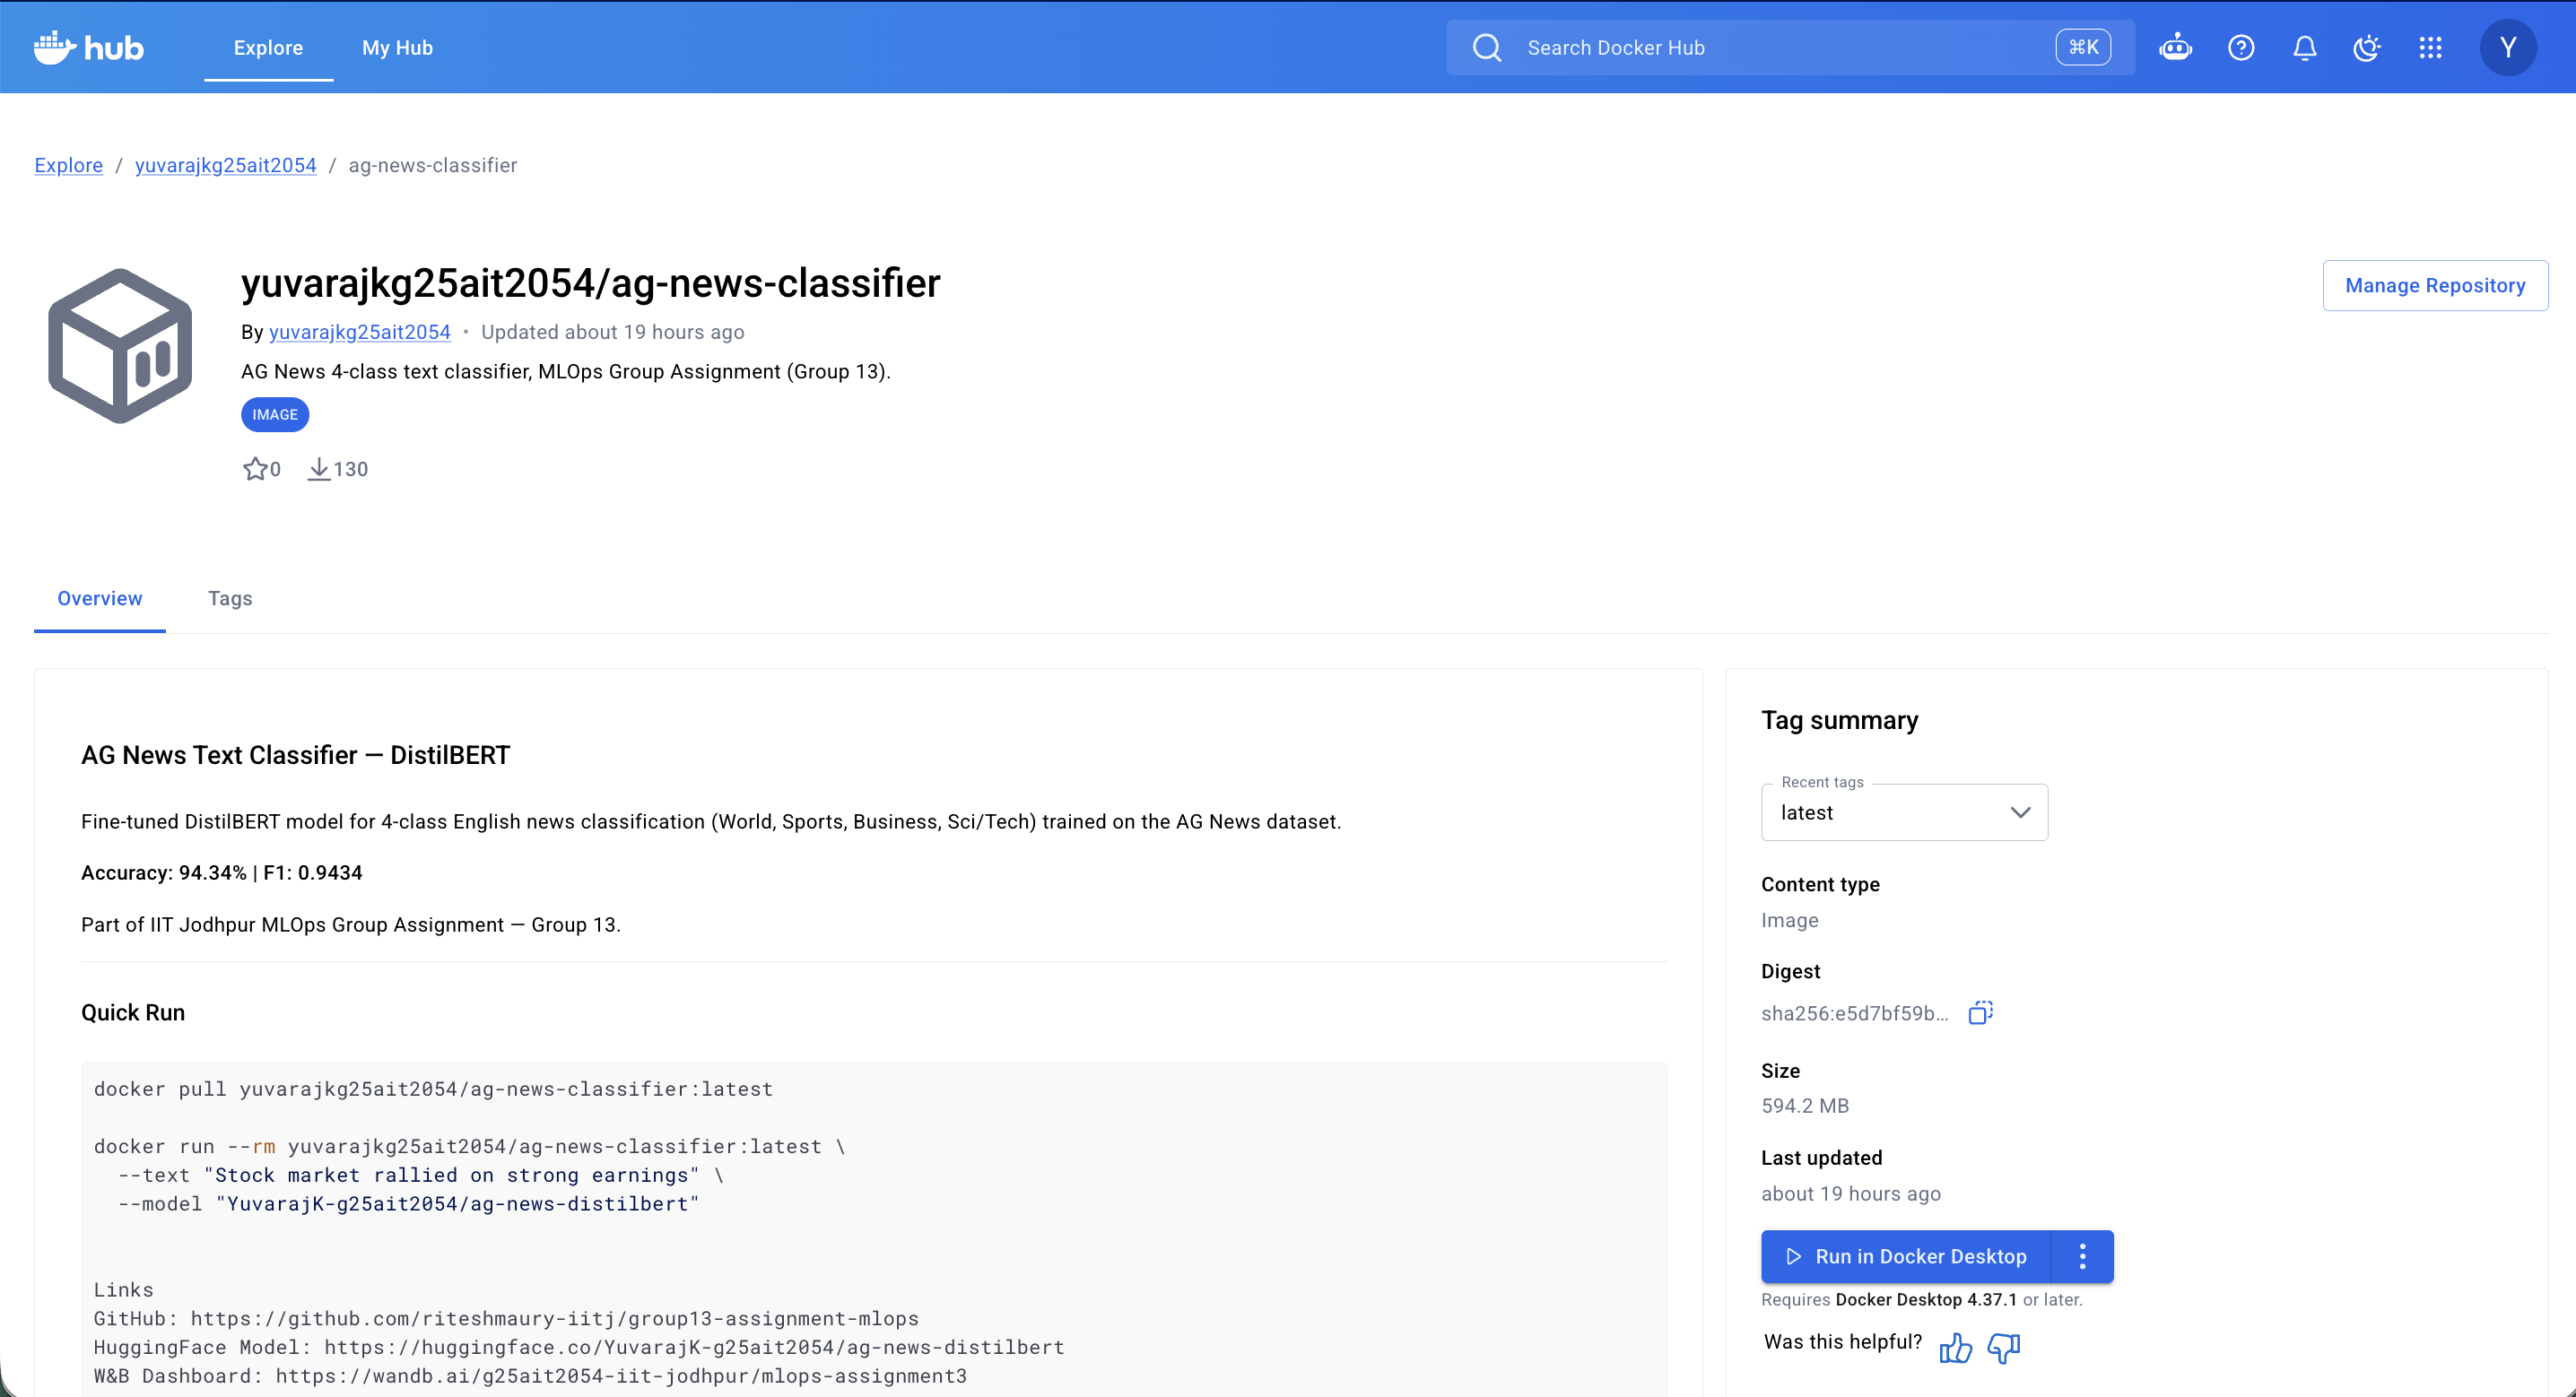
\includegraphics[width=0.85\textwidth]{screenshots/Docker_execution.png}
\caption{Inference workflow run log --- classification output}
\end{figure}

% ======================== PAGE 5 ========================
\section{W\&B Experiment Comparison and Conclusion (Task 8)}

\subsection{Task 8 --- W\&B Experiment Comparison [5 marks]}

The W\&B project is publicly accessible at:
\begin{center}
\href{https://wandb.ai/g25ait2054-iit-jodhpur/mlops-assignment3}{\texttt{https://wandb.ai/g25ait2054-iit-jodhpur/mlops-assignment3}}
\end{center}

The project contains runs \texttt{run-v1}, \texttt{run-v2}, and \texttt{push-model-v1} (logs HuggingFace model URL to W\&B summary).

\begin{itemize}[noitemsep]
  \item Version 1 (lr=2e-5, bs=16) converged smoothly; Version 2 (lr=5e-5, bs=64) had lower eval loss but slightly worse F1.
  \item Accuracy difference is small (0.22\%); Version 1 selected for deployment based on higher F1.
\end{itemize}

\begin{figure}[H]
\centering
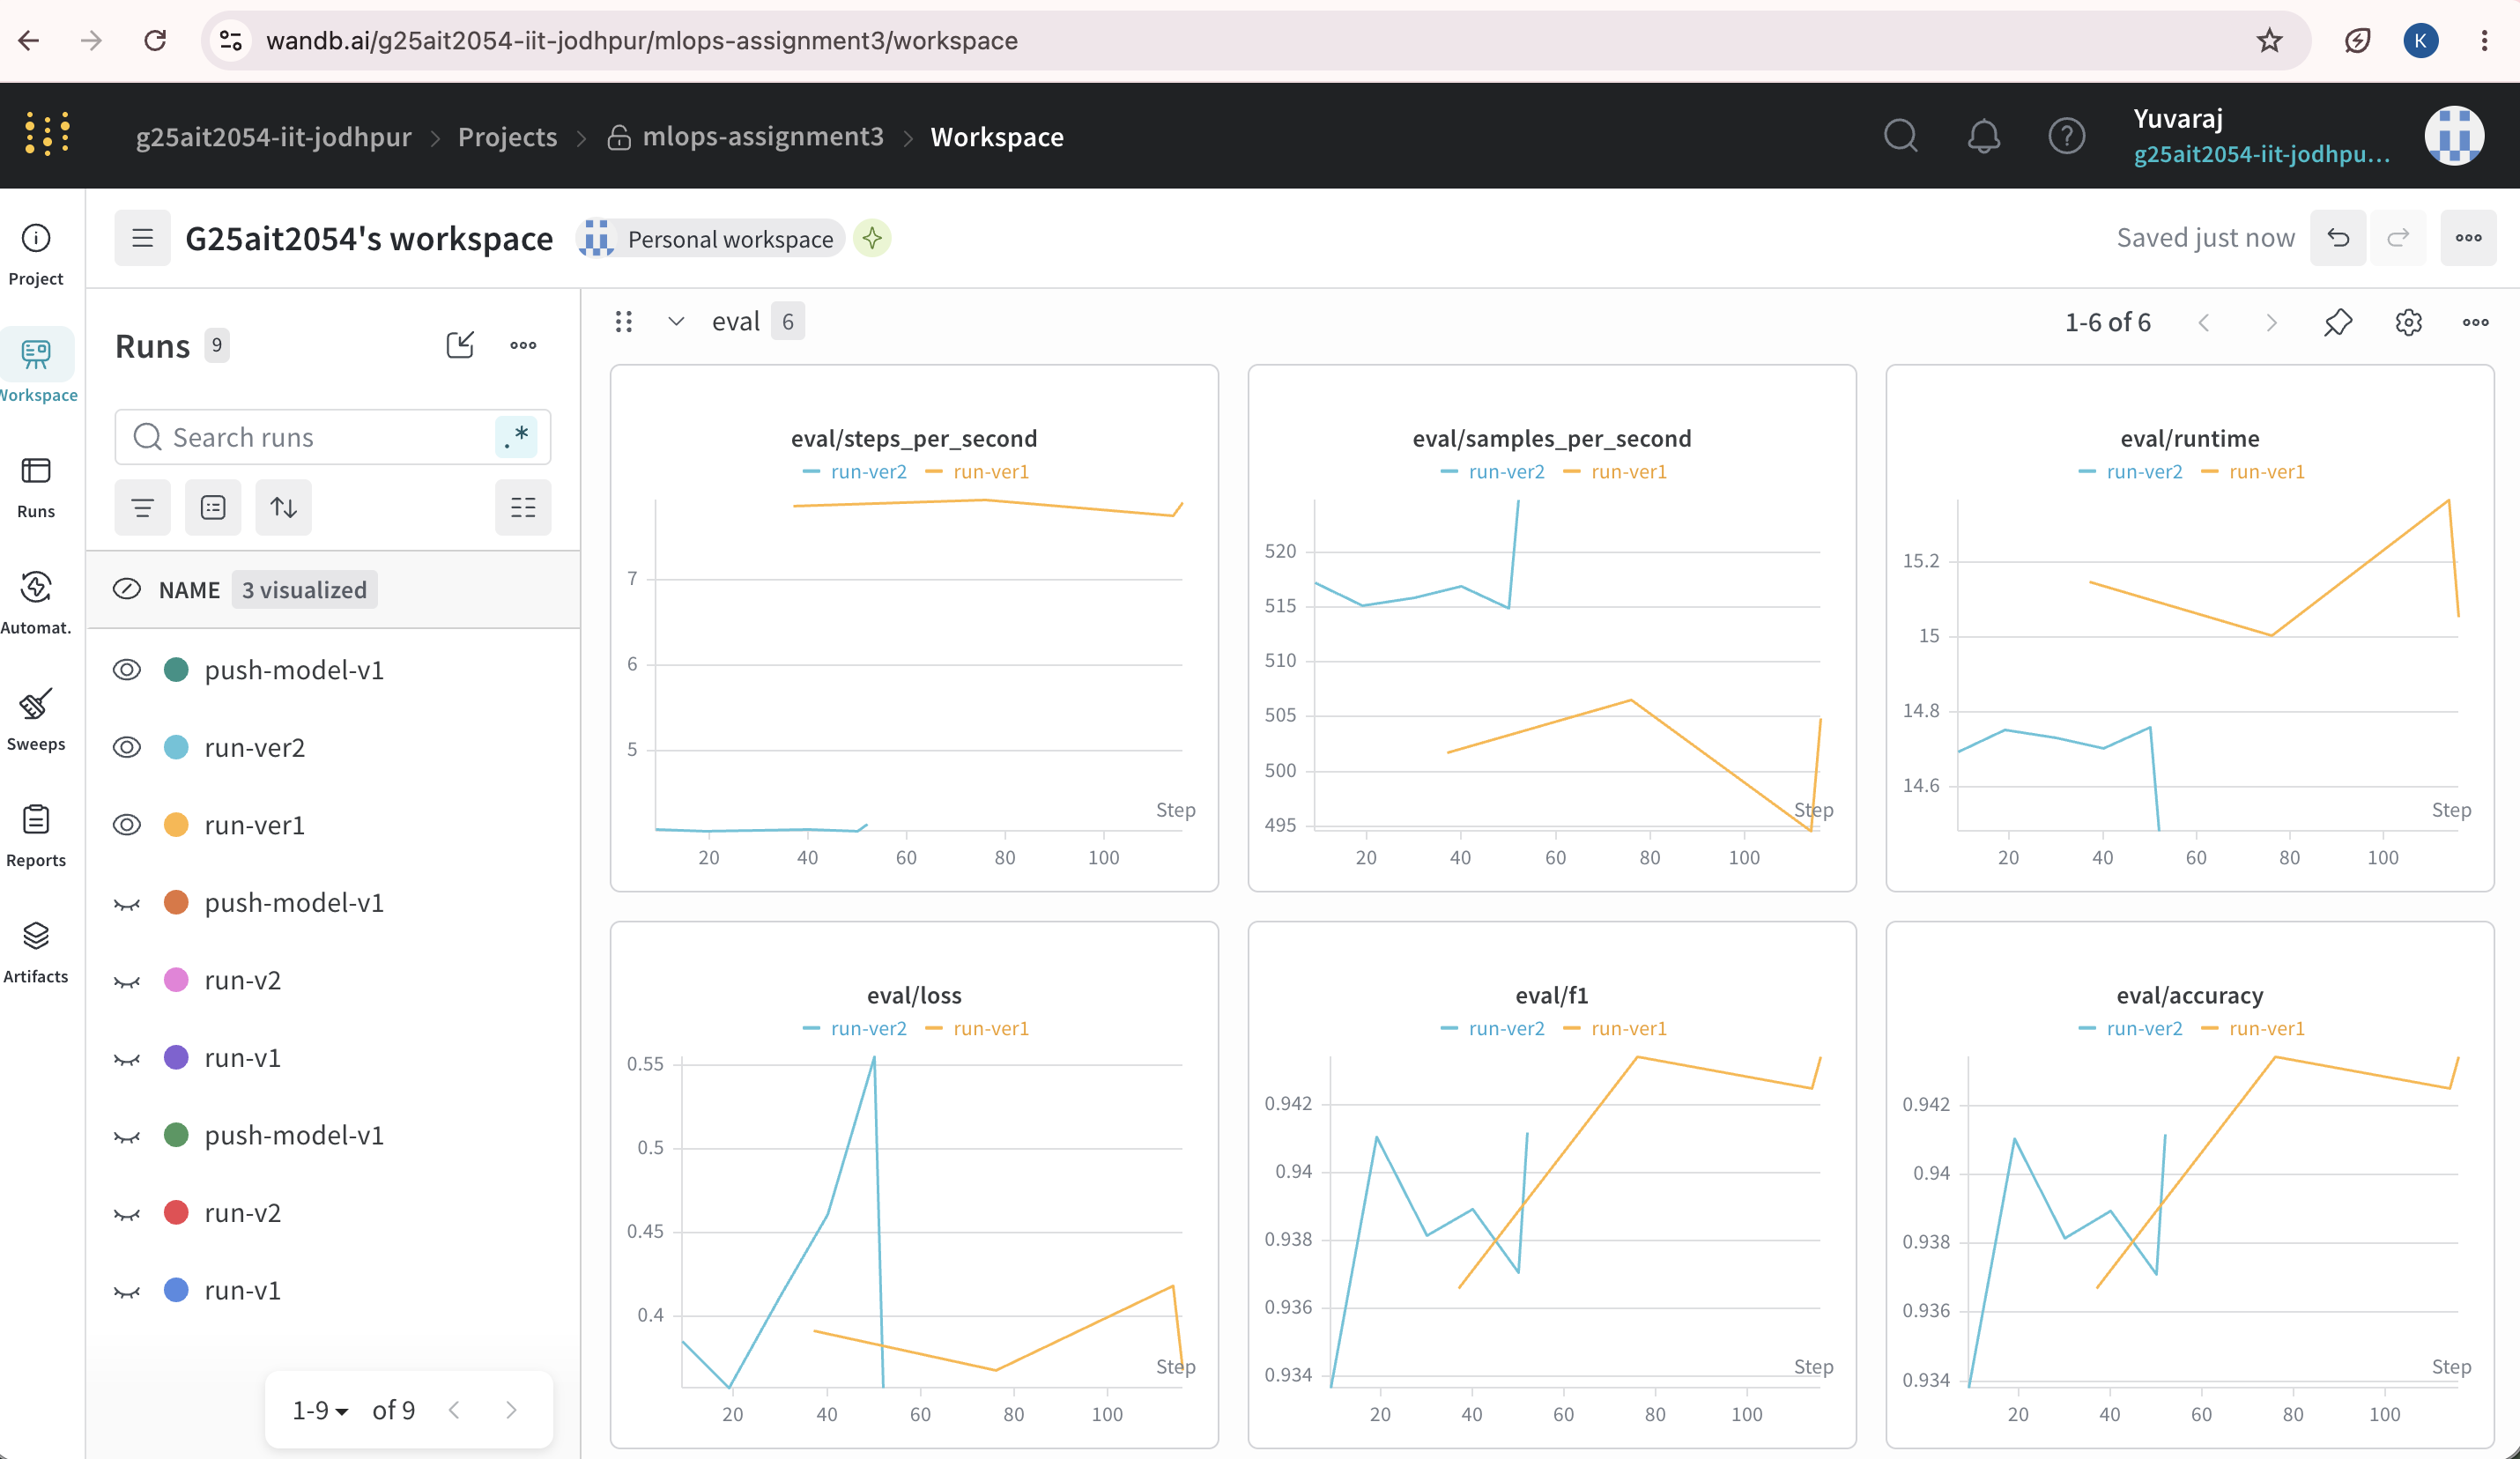
\includegraphics[width=0.85\textwidth]{screenshots/wandb_Eval.png}
\caption{W\&B runs table --- run-v1 and run-v2 with accuracy, F1, and loss}
\end{figure}

\begin{figure}[H]
\centering
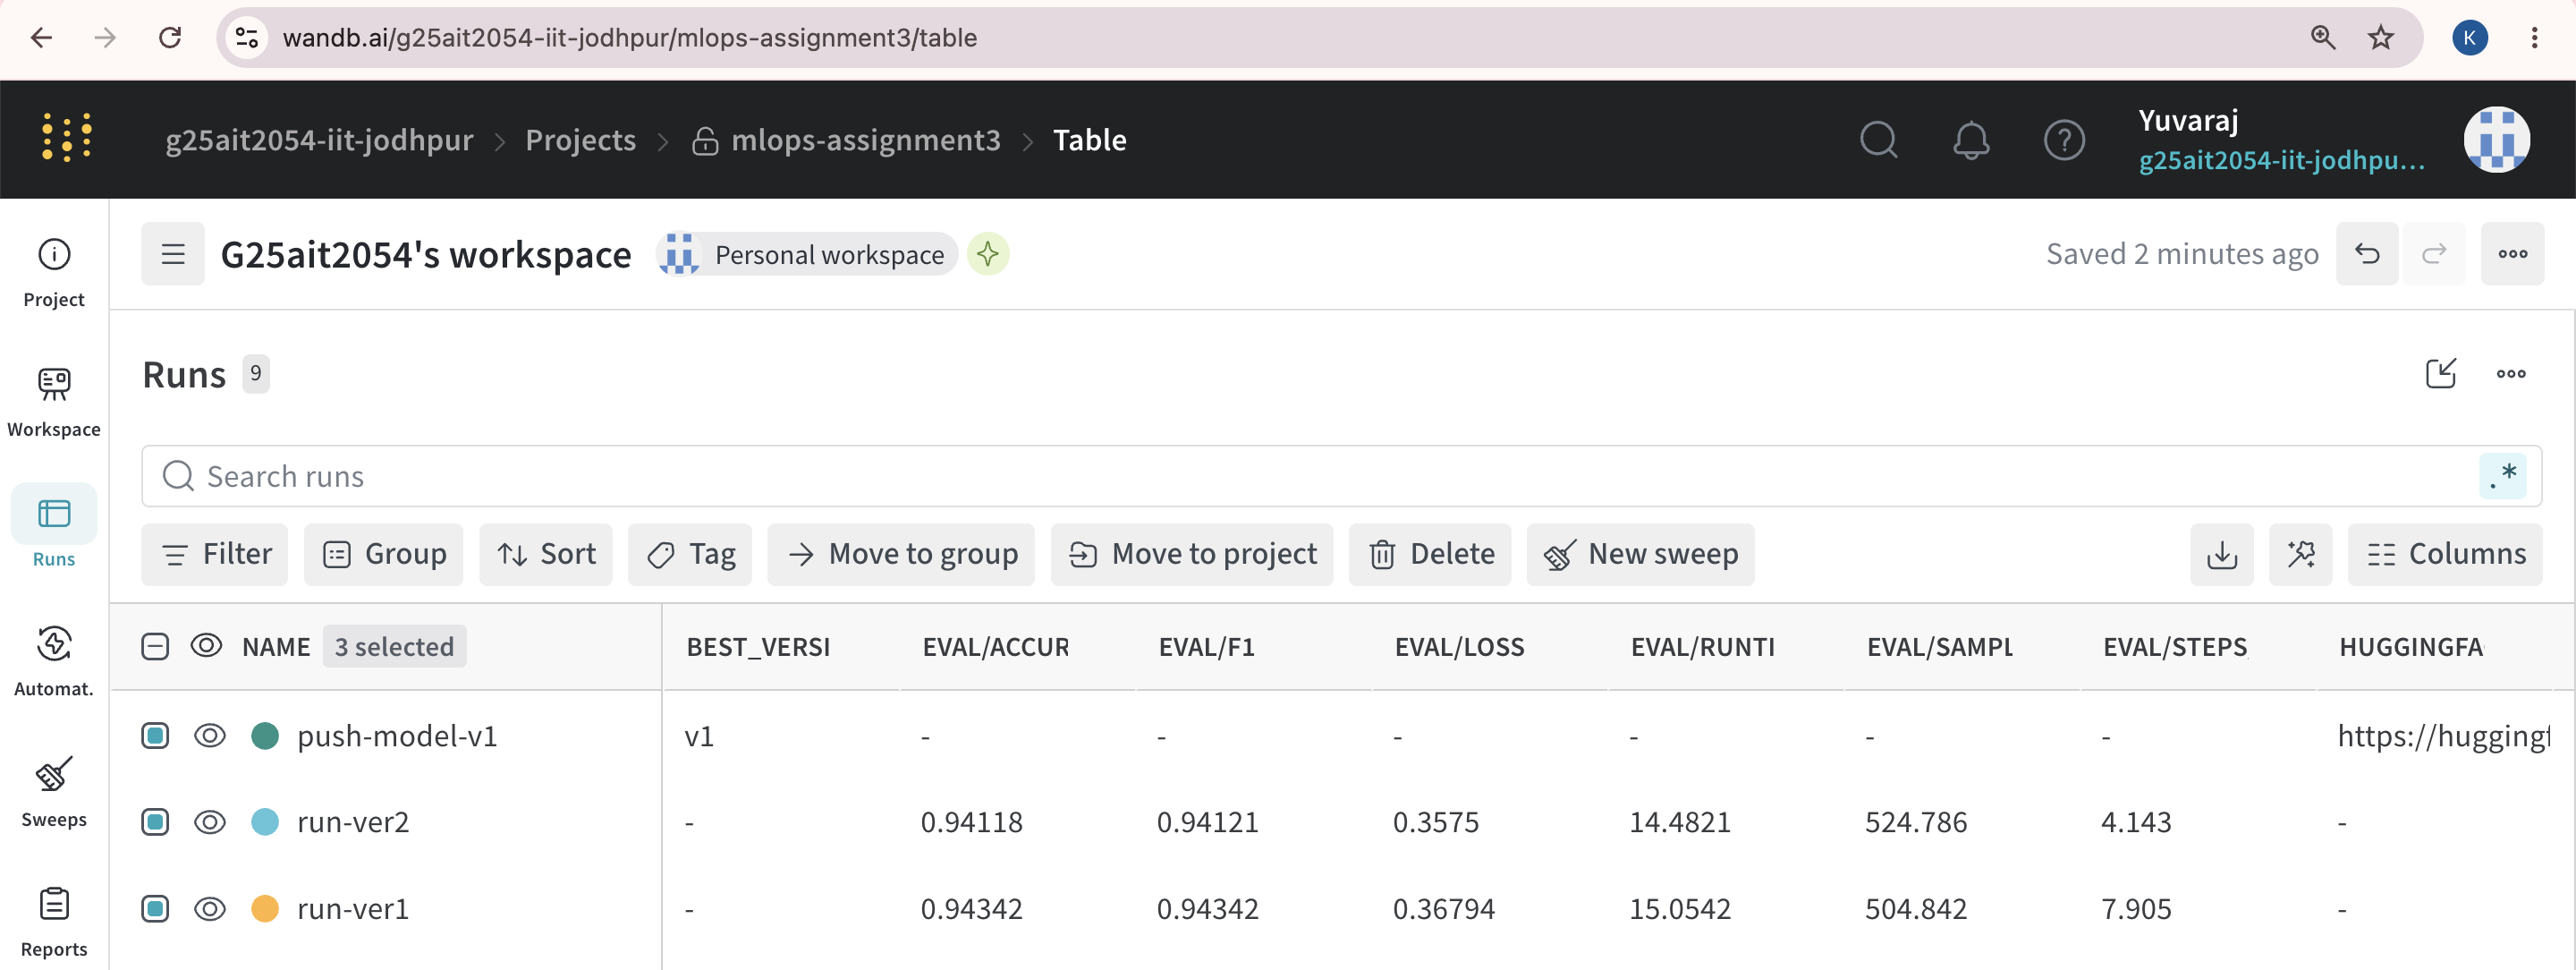
\includegraphics[width=0.85\textwidth]{screenshots/wandb_compare.png}
\caption{W\&B comparison view --- eval/accuracy and eval/loss with both runs overlaid}
\end{figure}



\subsection{Challenges}

\begin{itemize}[noitemsep]
  \item \textbf{Docker PyTorch:} Default PyPI \texttt{torch==2.5.1} has no CPU wheel; fixed by using PyTorch's CPU index URL (\texttt{2.5.1+cpu}).
  \item \textbf{DistilBERT token\_type\_ids:} DistilBERT does not use segment embeddings; had to remove \texttt{token\_type\_ids} from tokenizer output before model call.
  \item \textbf{GitHub Actions inputs:} \texttt{github.event.inputs} is empty on push triggers; fixed by hardcoding test values in the workflow YAML.
  \item \textbf{Merge conflicts:} Resolved by keeping \texttt{develop} versions of conflicted files.
\end{itemize}

\subsection{Summary of Deliverables}

\renewcommand{\arraystretch}{1.4}
\begin{tabular}{llll}
\toprule
\textbf{Task} & \textbf{Description} & \textbf{Status} & \textbf{Link / Artefact} \\
\midrule
Task 1  & GitHub Repo + Branching     & Done & \href{https://github.com/riteshmaury-iitj/group13-assignment-mlops}{GitHub} \\
Task 2  & Data Prep + Normalisation   & Done & \texttt{prepare\_data.ipynb} \\
Task 3  & Model Selection             & Done & \texttt{distilbert-base-uncased} \\
Task 4  & Training (v1 + v2) + W\&B   & Done & \href{https://www.kaggle.com/code/kyuvarajg25ait2054/group13-ag-news-k}{Kaggle} \\
Task 5  & HuggingFace Hub Push        & Done & \href{https://huggingface.co/YuvarajK-g25ait2054/ag-news-distilbert}{HF Hub} \\
Task 6  & Docker Image                & Done & \href{https://hub.docker.com/r/yuvarajkg25ait2054/ag-news-classifier}{Docker Hub} \\
Task 7  & GitHub Actions (CI + Infer) & Done & \href{https://github.com/riteshmaury-iitj/group13-assignment-mlops/actions}{Actions} \\
Task 8  & W\&B Comparison             & Done & \href{https://wandb.ai/g25ait2054-iit-jodhpur/mlops-assignment3}{W\&B} \\
\bottomrule
\end{tabular}

\end{document}
